\documentclass[12pt]{scrartcl}


\usepackage{hyperref}
\usepackage[pdftex,dvipsnames,cmyk]{xcolor}  % Coloured text etc.
\usepackage{upquote}
\usepackage{url}
\usepackage{appendix}
\usepackage{ifpdf}
\usepackage{placeins}
\ifpdf
  \usepackage[pdftex]{graphicx}
  \graphicspath{{graphics/}}
  \DeclareGraphicsExtensions{.pdf,.jpeg,.jpg,.png}
\else
  \usepackage[dvips]{graphicx}
  \graphicspath{{graphics/}}
  \DeclareGraphicsExtensions{.eps}
\fi

\usepackage[backend=biber,
            bibencoding=utf8,
            natbib=true,
            style=authoryear,
            hyperref=true,
            url=false,
            doi=false,
%            backref=true,
            maxcitenames=3,
            block=ragged]{biblatex}
\addbibresource{refs/thesisbibliointerimreport.bib}

\usepackage[colorinlistoftodos]{todonotes} % remove draft option in \documentclass to disable this package

\usepackage{listings}
\definecolor{pale-gray}{gray}{0.95}
\lstset{backgroundcolor=\color{pale-gray},language=SQL}
\usepackage{caption}
\captionsetup[lstlisting]{labelfont=bf}
\usepackage{abstract}
\usepackage[cache=false]{minted}
\usemintedstyle{colorful}
\setminted[sql]{frame=lines, framesep=2mm, baselinestretch=1.2, fontsize=\footnotesize, linenos}
\setminted[python]{frame=lines, framesep=2mm, baselinestretch=1.2, fontsize=\footnotesize, linenos}
% !TeX TXS-program:compile = txs:///pdflatex/[--shell-escape]

% See https://texfaq.org/FAQ-casechange
\usepackage[overload]{textcase}


\usepackage[toc]{glossaries}
\usepackage[utf8]{inputenc}
\makeglossaries

\newglossaryentry{Real}
{
    name=Real Energy Consumption,
    description={is the actual power consumed by the equipment to do useful work. It is distinguished from apparent power by eliminating the reactive power component that may be present}
}

\newglossaryentry{Reactive}
{
    name=Reactive Energy Consumption,
    description={is the actual energy consumed by the equipment to do useful work. It is distinguished from apparent power by eliminating the reactive power component that may be present}
}

\newglossaryentry{Apparent}
{
    name=Apparent Energy Consumption,
    description={is the combination of reactive power and real power is called apparent energy, and it is the product of a circuit's voltage and current, without reference to phase angle. Apparent energy is measured in the unit of Volt-Amps (VA) and is symbolized by the capital letter S}
}

\newglossaryentry{Power}
{
    name=Power Factor,
    description={(PF) is the ratio between 0 and 1 of real power (kW) to apparent power (kVA)}
}

\newglossaryentry{LCP}
{
    name=LCP Cooling Capacity,
    description={is the capacity of the Liquid Cooling Package to cool a rack in a Data Centre}
}


\begin{document}

\begin{titlepage}
	\newcommand{\HRule}{\rule{\linewidth}{0.5mm}}

	\center
	\textsc{\LARGE Waterford Institute of Technology}\\[1.5cm]
	\HRule\\[0.4cm]

	\huge\bfseries \MakeTextUppercase{Applying Data Mining Techniques to Monitoring Data from a Data Centre to Improve its Energy Efficiency}\\[0.4cm]

	\HRule\\[1.0cm]
	\textsc{\large Masters Dissertation}\\[1.5cm]
	\begin{minipage}{0.4\textwidth}
		\begin{flushleft}
			\large
			\textit{Student}\\
			John Fitzpatrick, 02323826
		\end{flushleft}
	\end{minipage}
	~
	\begin{minipage}{0.4\textwidth}
		\begin{flushright}
			\large
			\textit{Supervisor}\\
      Dr. Bernard Butler
		\end{flushright}
	\end{minipage}


	\vfill\vfill\vfill

	{\large\today}

	\vfill

\end{titlepage}

\newpage
\pagenumbering{roman}
\begin{abstract}
\renewcommand{\abstractname}{Abstract}
The growing prevalence of Data Centres and their associated services to commercial and individual consumers is an underlying feature of today's technological landscape. Therefore, as the energy consumed by these Data Centres is growing exponentially, efforts must be focused to maximise energy efficiencies in Data Centres in light of an ongoing global energy crisis. Existing literature in this regard focuses on physical improvements to server, networking or energy components as well as new management support systems.  This research identified a gap whereby the Data Centre is treated as an entity in its own right, combining its own operational monitoring data, that's collected on energy, weather and cooling systems and combining this with modern Data Mining techniques to uncover hidden insights that are richer and not seen from simple monitoring data. These insights could relate to predicting or explaining unexplained spikes in energy consumption or for explaining anomalies. This research specifically focused on the energy efficiency of the Chiller system in the WIT-TSSG Data Centre in Waterford. In particular, the research focused on the period of time before and after the operational Chiller alternated from Chiller 2 to Chiller 1, which saw unexpected spikes in Energy Consumption of Chiller 1. Correlation and Linear Regression analysis was carried out on the related variables (energy consumption of cabinets, weather information and cooling metrics) to identify the relationship between these variables and the operating chiller from week to week. Through this process, this research then identified certain variables that could indicate a potentially underlying issue, with the caveat that the full interpretation of these results will need input from Data Centre Engineers who understand the context of the underlying variables.       
\end{abstract}
\newpage

\section*{Acknowledgements}


Firstly I would like to thank Dr. Bernard Butler for all his support, guidance, knowledge and crucially patience in helping me complete this research. Without the skills and genuineness that Dr. Butler has brought to this project, it would not have been successfully completed. 

I would also like to thank John Ronan and Michal Kugel from the WIT-TSSG Data Centre for their time in meeting with me on multiple locations and for providing so much information on the Data Centre itself. 

Finally, I would like to thank my wife Sharon and daughter Lily for supporting me over the last year while this work was being completed. Again, without your support, this project would not have been possible.  

\newpage
\tableofcontents
\newpage
\listoffigures
\newpage
%\lstlistoflistings % needs the listings package
\newpage
\renewcommand\listoflistingscaption{List of Source Codes}
\listoflistings % needs the inbuilt listings environment of LaTeX; comment out the listings package stuff above otherwise nothing appears here
\newpage
\pagenumbering{arabic}

%\begin{document}

%\title{Thesis Proposal - Title TBC}
%\author{John Fitzpatrick}

%\maketitle

%\pagebreak



\section{Introduction}
\label{sec:[introduction]}
The demand for cloud computing services is growing exponentially, driven by the growth of internet users and applications (\cite{edssch.qt9c84f49g20130101}). As a result, within the Information and Communications Technology sector (ICT), Data Centres are the fastest growing sector in terms of energy consumption and are now responsible for over 2\% of the global CO2 emissions (\cite{edsbas.13818AC20170101}). With this growth in Data Centre energy consumption over the last 10 years, there arises a cost incentive, along with a general green incentive, to reduce energy consumption or to use energy more efficiently. While there is ample literature available that deals with making Data Centres more efficient by changing the hardware configuration of the Data Centre, this Dissertation documents the progress made on applying Data Mining techniques to the monitoring data, compiled from within a Data Centre, to unlock hidden information to assist system administrators to make the Data Centre more efficient or eliminate energy inefficiencies. Data from a medium sized Data Centre, the WIT-TSSG Data Centre in the Carriganore West Campus of Waterford institute of Technology is being used for this project.  


\subsection{Motivation}
\label{subsec:[Motivation]}
The goal behind making Data Centres more energy efficient is to reduce the energy consumption while delivering the same service to its users. Therefore the motivation that follows from this is twofold. 

Firstly, there is the motivation to make the Data Centre more energy efficient for the tangible benefits this brings. If energy consumption is reduced, this will lead to cost savings, while simultaneously reducing the carbon footprint of the Data Centre. Ultimately, this could deliver savings to WIT, allowing for potential investment in other educational projects while helping the environment at the same time. 

Secondly, in addition to the overarching motivation above, this research is being motivated by a desire to explore Data Mining techniques to gain insight into Data Centre energy consumption to help make them more energy efficient. While Data Centres are a part component of any cloud computing architecture, the emphasis here is to treat them as an entity in their own right, and use the vast amounts of monitoring data they generate to make them more energy efficient by highlighting energy inefficiencies. There is very little existing literature in this regard and the motivation here is that this study would contribute to the research in this field.  

\subsection{Research Problem Statement}
\label{subsec:[Research Problem Statement]}
As outlined in the introduction (section \ref{sec:[introduction]}), The information and Communication Technology (ICT) sector, and Data Centres in particular, are consuming vast amounts of energy and are contributing to an ever increasing carbon footprint.  \citet{edsbas.13818AC20170101} highlight that the ICT sector will consume 13\% of the global electricity supply by 2030. 

Therefore, as the energy demand of Data Centres grows due to the changing role of technology in society, this represents a clear challenge to policymakers, researchers and Data Centre stakeholders to seek solutions to make Data Centres more efficient in terms of energy consumption. 

A significant amount of research exists that focuses on making Data Centres more efficient, by concentrating on improvements to the physical hardware and infrastructure within a Data Centre. This, as detailed in the literature review, (section \ref{subsec:[Improving Data Centre Energy Efficiency]}) specifically focused on such measures as: 

\begin{enumerate}
	\item Introducing wireless sensors to capture key metrics;
	\item Following best practices and 
	\item Focussing on specific features within a Data Centre to gain efficiencies, such as the cooling system, server efficiencies, network modelling, or the optimisation of applications at an infrastructural level. 
\end{enumerate}

However, this research has a different focus. It analyses existing monitoring data, that is already stored by the Data Centre to seek hidden insights that might make a Data Centre more energy efficient. 

\subsection{Aims and Objectives}
\label{subsec:[Aims and Objective]}

The ultimate aim of this research, as specified in the Research Problem Statement (section \ref{subsec:[Research Problem Statement]}) is to use Data Mining Techniques on the monitoring data compiled at the WIT-TSSG Data Centre to gain hidden insights about energy consumption to help make the Data Centre more energy efficient. 
Specifically, the following are the aims and objectives of the project:

\begin{itemize}
\item Review all existing literature on improving Data Centre energy efficiency.
\item Learn about the WIT-TSSG Data Centre and what monitoring data is compiled that can be used for analysis.
\item Identify Data Mining techniques from existing literature that can be applied to the monitoring data compiled at the Data Centre.
\item Apply Data Mining techniques on the monitoring data from the Data Centre to maybe gain some hidden insights about energy consumption.
\end{itemize}

If successful with these aims, one objective is to understand when there is a peak in energy demand so that the supply of energy can be better utilized. Another objective arriving from ongoing discussions with staff from the Data Centre is to help identify known inefficiencies in the chiller system.  

If the project can meet these objectives, it will also have contributed to the academic literature on this subject, while simultaneously providing the Data Centre in WIT-TSSG with a predictive model to help better utilize the supply of energy at peak demand that in turn can lead to greater energy efficiencies, and assist in pinpointing specific problem areas of energy inefficiency within the Data Centre. 
 

\subsection{Research Questions}
\label{subsec:[Research Questions]}

From monitoring data provided by the WIT-TSSG Data Centre and using a Data Mining based approach,
\begin{enumerate}
  \item Can we identify features in the data that indicate where the Data Centre is not optimally consuming its supply of energy?
    \item Can we identify predictive indicators from the data that forecast an unanticipated peak in energy demand at the Data Centre?
  \item Specifically, can we identify energy or cooling features associated with the chiller system that are not energy efficient and could warrant remedial action.  


\end{enumerate}

The third Research Question was added in collaboration with system administrators in the Data Centre who had believed for some time that a potential issue was apparent in the Chiller system. While existing diagnostic techniques could not elaborated on any theory, feedback was provided in consultations with them, that this could be an area to concentrate on.      

\section{Literary Review}
\label{sec:[Literary Review]}

\subsection{Introduction}
\label{subsec:[Introduction]}

The literature review can be divided into three concepts. The first is an introduction to what Data Centres are, how they work and specifically an overview of the WIT-TSSG Data Centre in Carriganore in Waterford (section \ref{subsec:[Data Centre Infrastructure and the WIT-TSSG Data Centre]}).  

The next concept looks at the literature around improving the energy efficiency of Data Centres (section \ref{subsec:[Improving Data Centre Energy Efficiency]}). In most cases, the focus is on reducing energy consumption by improving the efficiency of different hardware components of a Data Centre. Specifically, that research looks at either the server, networking or cooling systems with an emphasis, by multiple authors, on implementing a wireless sensor system to capture key metrics across a Data Centre and using this to pinpoint issues in real-time. 

Other work in this area presents research on optimising resources or developing new scorecards to identify efficiencies in the management of Data Centres. 

The final concept looks at research on Data Mining techniques used to increase energy efficiency in buildings (section \ref{subsec:[Data Mining Techniques]}). There are numerous case studies using `Big Data' from building automation systems, to be harnessed in a Data Mining approach to identify hidden insights to improve the energy efficiency of different buildings. All three concepts are explored in detail below, before a summary ties all three concepts together and identifies the research gap that this project is investigating.        

\subsection{Data Centre Infrastructure and the WIT-TSSG Data Centre}
\label{subsec:[Data Centre Infrastructure and the WIT-TSSG Data Centre]}

\subsubsection{What is a Data Centre and How Much Energy do they Use?}
\label{subsubsec:[What is a Data Centre and How Much Energy do they Use?]}

In the modern economy, the demand for cloud storage and cloud computing based applications is growing exponentially as the number of internet users who rely on digital information via cloud services continues to sky-rocket across the world (\citep{VASUDEVAN201794}). To facilitate the demand in growth for such services, it follows that Data Centres, and the facilities they provide, will also be more in demand.  

\citet{edsdoj.99f37e7899fb4fcaabdaa81e395626c420180101} define a Data Centre as "a dedicated facility with all the resources required for storage, processing and sharing digital information and its supported areas".  The hardware required for such a facility comprises power distribution, environmental control systems, telecommunications, security and information technology (I.T) equipment~\citep{edsdoj.99f37e7899fb4fcaabdaa81e395626c420180101}. 

Figure~\ref{fig:DCenergy} from \citep{edsdoj.99f37e7899fb4fcaabdaa81e395626c420180101} outlines how energy is typically consumed in a Data Centre, specifically how it is channelled to IT equipment and non IT equipment.

\begin{figure}[h]
  \caption{How Energy is Consumed in a Data Centre.}
  \label{fig:DCenergy}
  \centering
    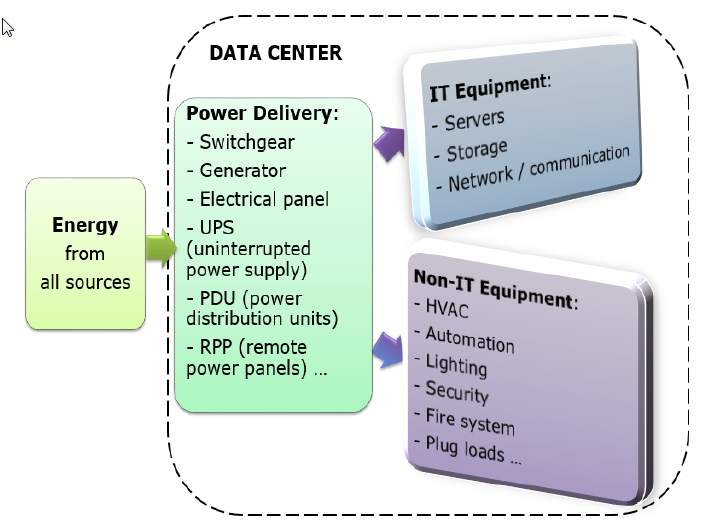
\includegraphics[scale=0.35]{Data_center_energy}
\end{figure}

%Currently, In terms of energy consumption, the entire Information and Communication Technology (ICT) sector including Data Centres now generates up to 2\% of the global CO2 emissions, which is on a par with the aviation industry.

Data Centres consume forty times more energy than conventional office buildings~\citep{edsdoj.99f37e7899fb4fcaabdaa81e395626c420180101} and have the fastest growing carbon footprint across the whole ICT sector~\citep{edsbas.13818AC20170101}.

Figure~\ref{fig:DCenergyEU-US}, reproduced from \citet{edsbas.13818AC20170101} shows the rising energy consumption of Data Centres across the EU and the US over the last 15 years as the number of Data Centres have grown:

\begin{figure}[h]
  \caption{Energy Consumption of Data Centres in the EU and US from 2000 to currently.}
  \label{fig:DCenergyEU-US}
  \centering
    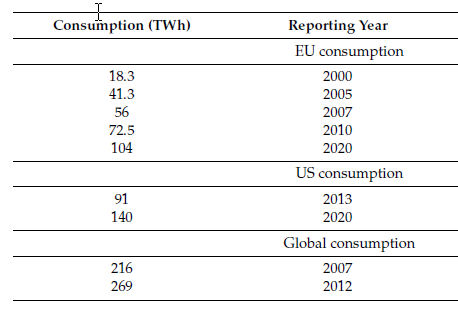
\includegraphics[scale=0.45]{Energy_consumption}
\end{figure}

With Data Centres consuming more energy, there is an obvious incentive, both from a cost and a green perspective, to reduce energy consumption per Data Centre. This can be done by making Data Centres more efficient for the energy they consume and the measurement that is used to measure energy efficiency is the \emph{Power Usage Efficiency} (PUE) score. This is described as

\begin{quotation} 
Power Usage Effectiveness = Total Facility Energy Usage/ IT Equipment Usage.
\end{quotation}

Lower PUE scores are better, and a PUE close to one indicates that the Data Centre is more efficient as it consumes less energy on non IT equipment such as cooling. 
In terms of the current trends of energy usage, research by \citet{edsbas.13818AC20170101} show that Data Centres in Northern Europe have a lower PUE score than those in southern Europe, which is expected given the geographical and climate difference. Also, the same authors find that the PUE scores in general have been decreasing year after year as demonstrated by the graphs in Figures \ref{fig:PUE-by-location} and \ref{fig:PUE-by-year}.

\begin{figure}[h]
  \caption{The average PUE across different locations.}
  \label{fig:PUE-by-location}
  \centering
    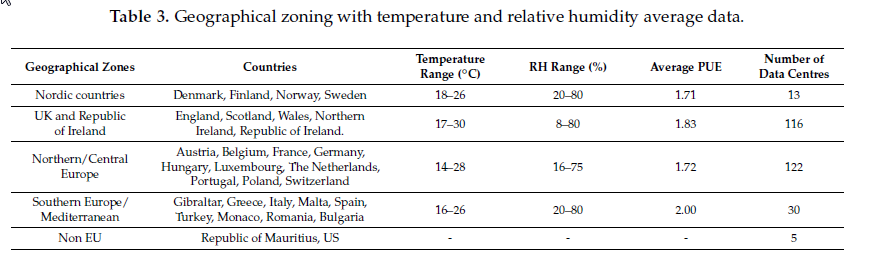
\includegraphics[scale=0.45]{geographical_zoning}
\end{figure}

\begin{figure}[h]
  \caption{The average PUE from 2000 to currently.}
  \label{fig:PUE-by-year}
  \centering
    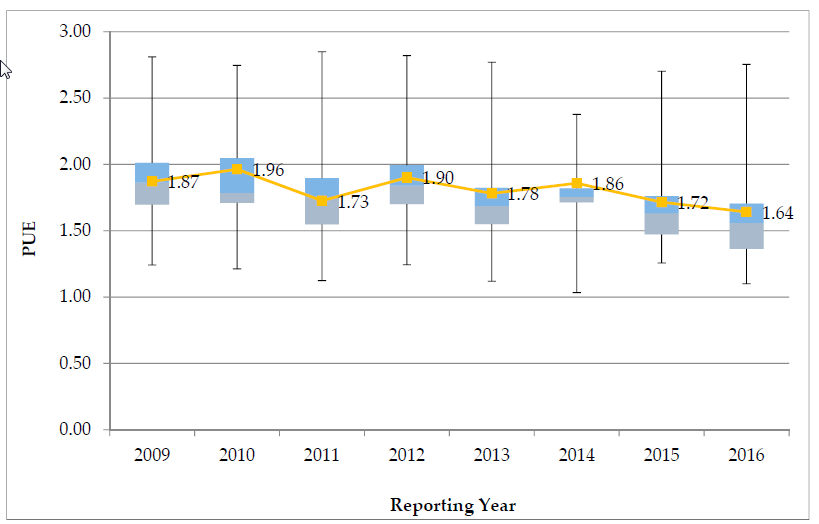
\includegraphics[scale=0.35]{Average_PUE_per_reporting_year}
\end{figure}
 
So the challenge, as outlined in the various literature below (section \ref{subsec:[Improving Data Centre Energy Efficiency]}), is how to make a Data Centre more energy efficient by eliminating energy inefficiencies within the IT equipment to reduce the consumption of energy overall. 

\subsubsection{The WIT-TSSG Data Centre}
\label{subsubsec:[The WIT-TSSG Data Centre]}

The WIT-TSSG Data Centre is located on the Carriganore West Campus of the Waterford Institute of Technology (WIT) on the west side of Waterford city. From this location, the Data Centre supports over 50 concurrently active ICT research projects through provisioning of internet services, Cloud Computing resources, an AI cluster and project bespoke test beds \citep{TSSG}. 

In particular, the Data Centre supports TSSG projects, the Higher Education Authority, The Irish Centre for High End Computing(ICHEC), hosting its super computer Kay, Arclabs and other 3rd party commercial arrangements.

In terms of its energy usage, the Data Centre has an IT power load of 300kW, with cabinets engineered to house 30kW of IT equipment. 1+1 300kW UPSs and an 800kW Generator provide the backup power \citep{TSSG}.

With regards to physical hardware, the Data Centre supports over 160 physical servers, providing more than 1,000 cpu cores for processing and 400 virtual servers for cloud computing.  In addition, there is over half a PB (that is 512 TB) of Data Storage, and ~3,000 network port \citep{TSSG}. 

Figure~\ref{fig:TSSGdataCentreDesign}, provided from \citet{TSSG} demonstrates the design and infrastructure of the Data Centre building.  

\begin{figure}[h]
  \caption{The design of the WIT-TSSG Data Centre.}
  \label{fig:TSSGdataCentreDesign}
  \centering
    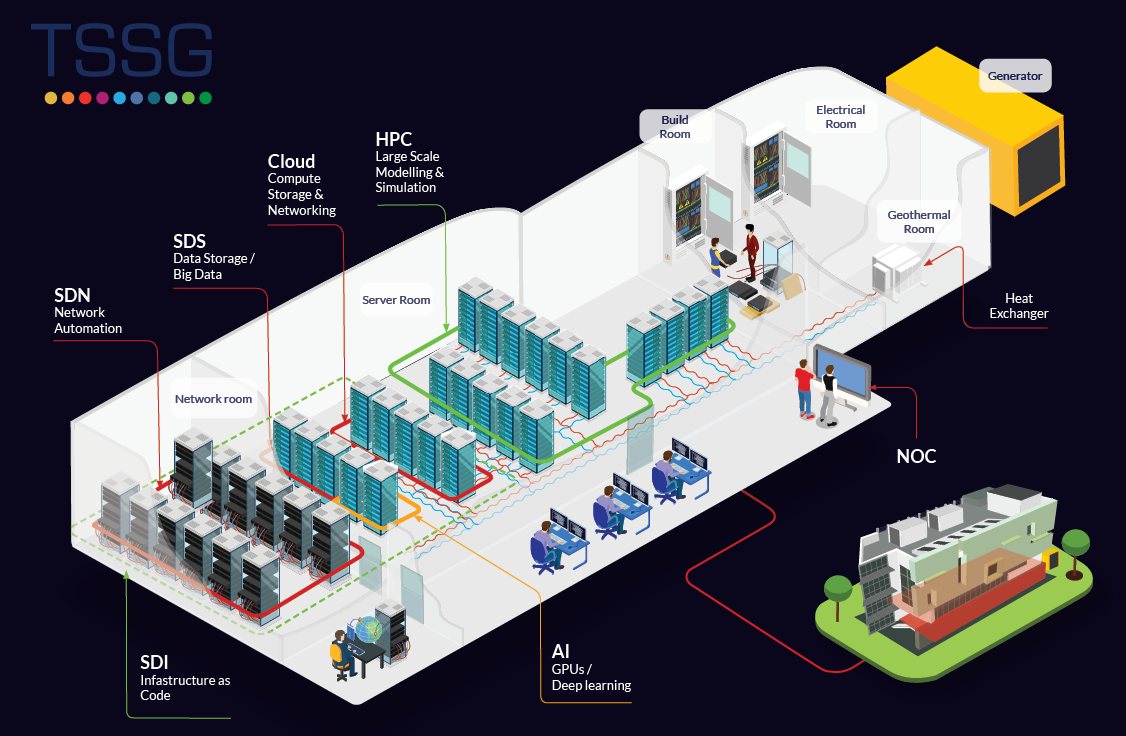
\includegraphics[scale=0.35]{TSSG_Diagram}
\end{figure}

This diagram illustrates that there are 26 Cabinets and these use varying degrees of KW per cabinet to house over 160 servers. In addition, the Data Centre is designed so that there are separate rooms for servers, networking equipment, UPS and batteries with the generator and cooling equipment outside. This is to optimise the best cooling option for each room, resulting in the server room not having any hot or cold aisles. Instead, all heat and cooling is contained inside the 26 cabinets \citep{TSSG}.

In terms of a cooling system, the Data Centre uses a water based cooling system which uses less energy than an air cooled system. There are two Chillers in the Data Centre who operate alternate weeks. For monitoring and visualisation, the Data Centre uses Nagios and the ELK software stack \citep{ELK} with the output from that monitoring system is discussed further in section \ref{subsec:[Data Available]} and \ref{subsec:[Exploratory Data Analysis]} (Data Available and Exploratory Data Analysis). 

Also, as part of this research, several Data Administrators at the Data Centre were interviewed to garner further information on the Data Centre. They were able to identify specific features that might warrant investigation and outline current projects to upgrade the Data Centre while they also outlined any anomalies I might expect to see in the monitoring data.  

In addition to this, when conducting the correlation analysis as outlined in section \ref{subsubsec:[Analyse Correlations]}, it became clear that further understanding was needed of the metrics involved and how energy consumption might be measured in a Data Centre. \cite{edseee.792155120170101} provide a comprehensive set of metrics and key performance indicators that are used in Data Centres that can be used to add context to the analysis of the WIT-TSSG Data Centre. 


\subsection{Improving Data Centre Energy Efficiency}
\label{subsec:[Improving Data Centre Energy Efficiency]}

From the Research Problem Statement (section \ref{subsec:[Research Problem Statement]}), the benefits for improving Data Centre energy efficiency is twofold: reducing the carbon footprint of the Data Centre, and reducing the cost of maintaining the Data Centre and these benefits should be mutually inclusive. Therefore, with such a desired outcome at stake, it is not surprising that a large amount of literature devotes itself to efforts in improving energy efficiency in Data Centres.

As outlined from the previous section (\ref{subsec:[Data Centre Infrastructure and the WIT-TSSG Data Centre]}), Data Centres are recent innovations, so to a degree, the literature is still catching up with the newest technologies and best practices. However, it is important to outline the earlier literature to understand why modern Data Centres, such as the WIT-TSSG Data Centre would have the ability to capture and store sensory data from its general operations. The following research summarises the need for such a sensor system and the immediate benefits this can bring to the energy efficiency of a Data Centre.   

To begin, a study by \citet{edsbas.A50BA51A20120101} states that implementing a sensor system to capture data can reduce energy demand by as much as 80\% through aggressive pursuit of energy efficiency measures specifically focussed around servers. The authors also provide a model to estimate efficiency potentials associated with discrete efficiency measures applied to different types of IT equipment., 

While in 2013, the literature from this time also calls for the implementation of wireless sensors to begin capturing data. Here, \citet{edssch.qt9c84f49g20130101} argue that capturing this data via wireless sensors and then using integrated software to manage and integrate this into management systems can allow for greater efficiencies in a Data Centres cooling system and power usage. Specifically, the paper suggests that by implementing such measures, Data Centres could reduce energy by as much as 17\%, with specific savings within this attributed to the cooling energy.

\citet{edsjsr.4134817120120101} also explain that a lack of visibility into a Data Centres operating conditions is an underlying reason for low-energy utilization. In this study, the authors argue for the introduction of sensor networks that combined with modelling, could provide insights into the distribution of energy and resolve the tension between cooling and performance, highlighting how the relationship between workload placement, performance and total energy is poorly understood.    

While these outlined the immediate and obvious benefits of integrating more reliable monitoring data into management systems and decisions, which by and large has been implemented, more recent literature investigates where more marginal gains can be found.  

\citet{edsdoj.47fdd5c4e23a43e3aa37ddd2fb75d82b20160101} looks to the performance of network capabilities and in particular, this research develops simulation models to predict the performance of networks based on the traffic through networks. It concludes that while the  network performance models developed by the authors only leads to minor prediction accuracy degradation, the same models can however, accelerate the performance analysis by a much larger factor. 

\citet{edsarx.1402.080420140101} use sensor data and a Map-Reduce computation in Hadoop to analyse server usage to maximise the efficiency of CPU power being used by each server in a Data Centre, thereby introducing some advanced data analysis of a specifically gathered sensor data. This introduces a measurement-based characterisation of energy consumption in a server and concludes that CPU consumption is neither linear or concave with the load within a server. 

\citet{edsbas.DFD37F4F20160101} moved the argument on from creating sensor networks to developing a monitoring service for energy efficiency and sustainable management in Data Centres. The approach the authors use is to collect the monitoring data, analyse the data captured and then execute based on the outcome of the analysis. This study concluded that such an approach is an adequate platform to contain a monitoring service offering a robust solution. This is further developed today in Data Centres where centres use the TICK or ELK (section \ref{subsubsec:[The WIT-TSSG Data Centre]}).  

Another approach used to improve Data Centre energy efficiency in the literature is advanced by \citet{edsdoj.99f37e7899fb4fcaabdaa81e395626c420180101} who introduce a whole new set of metrics to review the efficiency of Data Centres. They argue that while the old metrics are valuable, some key metrics concerning \emph{risk} are overlooked. They advance a new Data Centre multidimensional scorecard which gives better visualisation to identify areas of improvement and crucially, standardise a process that could eventually become best practice and allow for true comparisons Data Centres. 

More advanced initiatives are based around the optimisation of physical resources within a Data Centre. \citet{10234066620151001} propose a multi-tier architecture-orientated virtualised application performance model to allocate computing resources to each machine based on SLA (service level agreement) restrictions. The authors develop a heuristic mixed optimisation algorithm to achieve this and the study finds that the proposed method is efficient in improving the overall performance and reducing the energy cost of the Data Centre.

Finally, \citet{VASUDEVAN201794} seek to reduce the operational costs of Data Centres and maximise energy efficiency by analysing log data to profile applications using the Data Centre. In addition, the authors profile the virtual and physical machines in the Data Centre, and using a penalty-based matching algorithm match different applications with the most compatible machines (virtual and physical) so that CPU usage is more efficient. Through experimental studies, the study concludes that such a profiling approach is feasible, scalable and energy efficient.

The literature outlined here demonstrates the changing focus of how best to increase the energy efficiency of data centres. From early research, just ten years ago, seeking the implementation of sensor systems that would lead to improved management systems and easily identified gains, to more recent and more advanced techniques looking to use algorithms to increase optimisation of the resources in a Data Centre. In all cases highlighted, the importance of capturing, understanding and using data to integrate new information into management systems and operations is stressed. However, in these instances, the approaches identify explicit data they want to capture and analyse, whether this is log data on CPU utilization or specific monitoring data. In general, few Data Mining approaches are used, in the sense of using implicit data to uncover hidden insights. The research questions in section \ref{subsec:[Research Questions]} focuses on this concept.  


\subsection{Data Mining Techniques (for improving energy efficiency in buildings)}  
\label{subsec:[Data Mining Techniques]}
Data Mining is the process of uncovering hidden patterns from large sets of data, where the data is analysed to extract information which can be transformed into valuable knowledge for the future. Such techniques include statistical and machine learning techniques which take the form of regression analysis, classification, cluster analysis and more advanced techniques such as neural networks. These techniques analyse the relationship between variables to uncover such hidden patterns and trends.  

While there is limited literature or existing research on using Data Mining techniques to improve the energy efficiency of Data Centres, there is comprehensive research on using Data Mining approaches to assess the energy efficiency of buildings in general, or of various systems within buildings. Because a Data Centre is a building in its own right, it is important to review such Data Mining techniques in the building management literature and assess if the research can be applied to Data Centres.   

In general, the literature can be divided into two sections, where basic Data Mining techniques are used, as described above, and when more complex algorithms are used to gain insights. First, I explore the literature on the basic Data Mining approaches.
 
\citet{XUE2017926} look at district heating substations in Northern China, and from operational data collected from the substations, use clustering techniques to identify seasonal and daily operating patterns, and association rules mining to identify faults, malfunctions and inefficient operations strategies. Using data from the meter reading system, the authors conclude that the Data Mining techniques can extract potentially useful knowledge in terms of fault detection and operation optimisation. 

\citet{JEFFREYKUO2018120} use regression and classification techniques on different factors in analysing the energy consumption characteristics of Taiwan's convenience stores. The data is collected from a survey of convenience stores owners before the Data Mining techniques look at intercorrelation between energy consumption and other factors such as geography, climate and store design. The knowledge obtained through these techniques can ultimately provide the owners of the stores with design decision mechanisms in line with the findings.  

Also, using monitoring data from building automation systems, \citet{FAN2018296} explore how unsupervised Data Mining techniques such as clustering, association rule mining, motif discovery and unsupervised anomaly detection can be used to gain insights into energy efficiencies within buildings. Here the authors review and summarise the techniques used and elaborate on the challenges and opportunities of using each and acknowledge that this is still a developing area of study.  

In another paper by the same authors, and using operational data from the construction of an education building in Hong Kong University, \citet{FAN2018296} use decision trees, motif discovery and gradual pattern mining to uncover novel and valuable insights for the management of energy consumption for the building. The paper highlights how these insights on building operational characteristics which can be obtained to pursue fault detection and optimal control strategies can be developed to enhance building operational performance.   

In a similar study by \citet{ZHOU201873}, the authors use data supplied from heat supply companies in Singapore and look at the correlation between energy consumption and building physics, the heating system and room position. The authors use the information gain ratio algorithm and decision tree classifiers to analyse energy consumption and other related factors and their main conclusion being that this a promising approach for such analysis. 

\citet{AHMAD2018460} use Gaussian process regression, multiple linear regression, tree bagger, bagged tree, boosted tree and neural networks to identify abnormal behaviour and predict the future heating and cooling demands in building environments. The results from this study showed that the six models were efficient in foreseeing anomalies and predicting the future heating and cooling demand in the building environment.  

These approaches will be reviewed when finalising a predictive model for energy consumption in section \ref{subsubsec:[Construct Regression Model]}. However, in addition to those highlighted, further literature has been sourced that specifically concentrated on analysing energy consumption in a Data Centre. \citet{Makris2017} collects data from the Data Centre processor, access memory and the network interface controller and analyses these features using linear regression to predict energy consumption at a system-level.

A precursor to the regression analysis is correlation analysis as outlined in section \ref{subsec:[Correlation Analysis of Chiller 1 versus Chiller 2]}, and it was important to understand the value this can bring to a data mining approach. \citet{13375977120180401} use multivariate correlation and data mining clustering techniques for detecting distributed denial of service attacks in cloud computing. Specifically, the authors investigate the correlation among selected and ranked variables. Such an approach is used in this project to identify predictive features of energy consumption and pinpoint potential inefficient energy consumption.    

However, some research also uses more advanced algorithms to gain hidden insights from the data captured. 

\citet{13090171620180801} use log data and the self-organising maps algorithm to create a decision support application for anomaly detection in IT systems. They highlight that this algorithm is used in anomaly detection in fraud cases and security attacks, but most importantly they highlight, when using the log data from systems, the self-organising maps algorithm allows for early detection of failures in critical systems in real-time. 

The Random Forrest Algorithm is used by \citet{WANG2017251} to discover critical events for event driven optimisation in building air-conditioned systems. With data collected from the building automation system, the authors make a case for using Data Mining to gain efficiencies in air conditioned systems by moving away from a time based system, to a more event driven optimisation.  

The literature reviewed at this point highlights the wide and varied Data Mining approaches taken by various authors to gain hidden insights into energy efficiencies within buildings or building systems such as heating or cooling systems. 

This project will adapt these approaches to the monitoring data we have gathered from WIT-TSSG Data Centre to help answer our Research Questions (section \ref{subsec:[Research Questions]}).   

\subsection{Summary}  
\label{subsec:[Summary]}
The research questions (section \ref{subsec:[Research Questions]}) clearly set out the goal of maximising energy efficiency within a Data Centre and the literature review sets out the framework for building the foundations for this research. Firstly, it defines what a Data Centre is and what the trends are in energy consumption by Data Centres (section \ref{subsubsec:[What is a Data Centre and How Much Energy do they Use?]}) before introducing the WIT-TSSG Data centre in Waterford (section \ref{subsubsec:[The WIT-TSSG Data Centre]}). From these foundations, the literature review focussed on various computational and systematic improvements that could lead to greater energy efficiency within a Data Centre (section \ref{subsec:[Improving Data Centre Energy Efficiency]}). The importance of wireless sensory data is a common starting point for most authors who focus on efficiency improvements to be made by concentrating on hardware improvements (network, server or cooling systems). Most of these approaches use data which is specifically captured at a system level to assist the goal of increased energy efficiency.

This is where I believe there is a research gap. Data Centres are entities in their own right and store vast amounts of operational and monitoring data. This has been harvested by a monitoring system and could be useful to analyse, using Data Mining techniques, to find hidden insights around energy efficiency or to find instances of where energy is being used inefficiently. 

Based on this, the final section of the literary review looked at where Data Mining techniques are used for similar applications (section \ref{subsec:[Data Mining Techniques]}) such as the energy efficiency of different building types, or heating or cooling systems within a building. Various Data Mining techniques are explored in the literature and are assessed to see if such approaches can be adapted for use in a Data Centre.   

\section{Methodology}

\label{sec:[Methodology]}

The literature review (section \ref{sec:[Literary Review]}, identified a gap where data mining techniques could be used on the monitoring data compiled within a Data Centre to unlock hidden sources of information that could lead to greater energy efficiency in operating the Data Centre. The research questions (section \ref{subsec:[Research Questions]}), ask if these efficiencies could brought about by identifying anomalies in the Data Centre where energy is not being used efficiently, with specific focus on the Chiller system and also looking to predict when energy demand peaks in order to better utilise the supply of energy that the Data Centre.

 

Whereas the majority of literature analyses the hardware components of a Data Centre to improve efficiency (section \ref{subsec:[Improving Data Centre Energy Efficiency]}), this research proposes to concentrate on monitoring data that tracks energy demand in the Data Centre to gain insights to unanticipated spikes in energy demand. There are two elements to this, analysing when the demand of energy consumption spikes, and analysing how the Data Centre manages that demand. 

 

At any given time, a Data Centre will have a certain load to process, and will utilise its available resources to process the load. To maximise efficiency therefore, a Data Centre would need to be able to best match the energy demand with the supply at its disposal. The real gains in efficiency therefore, is to be able to anticipate and understand the demand to best utilise the resources at its disposal. In technical terms, this would mean moving loads between racks within a Data Centre or reducing the demand for the cooling system at certain times. Therefore, to increase the efficiency of a Data Centre by concentrating on energy demand, we need to anticipate the demand of energy usage or identify inefficiencies in the system that was causing such a demand for energy.

 

The approach taken to achieve this, after consultation with Data Administrators in the Data Centre is to concentrate on the performance of both Chillers. They believe, but had no direct evidence, that the Chiller system is currently not energy efficient. Preliminary analysis (section \ref{subsec:[Aims and Objective]}) indicated that indeed, at certain times of the year there was unexpected spikes in energy consumption of Chiller 1. Therefore, this project would focus on those spikes, to both identify and understand the sudden spike in energy consumption and to potentially find relating factors that might be related to this. To do this, this Dissertation will use correlation analysis to identify predictive features of energy consumption and follow this with regression analysis to build a predictive model of energy demand.

 

Firstly, correlation analysis is used to identify the relationship between the Chiller system and other energy indicators. As there are two Chillers in the Data Centre, with each Chiller operating on alternating weeks, we can use correlation indicators to view the relationship between the Chiller in operation for one week and other measures for that week such as weather variables, the temperature of the water leaving the cooling system or the energy demand of different cabinets and servers. In theory, allowing for weather factors, the relationship between a Chiller and the other variables, which is measured as a correlation co-efficient, should be stable from week to week, regardless of the Chiller in operation. Therefore the correlation analysis will identify particular variables that are different from week to week.

 

From this, and using the variables identified by the correlation analysis, and controlling for other factors such as the weather, a linear regression regression model will be built that charts the relationship between those variables identified and the chiller in operation for a certain week. This is essentially a predictive model of energy demand for a chiller for a particular week. So we can measure the coefficients of these variables week to week, so identify variables that are statistically different. The basic model takes the form of:

\begin{equation}
\hat{Y}_i = \hat{\beta}_0 + \hat{\beta}_1 X_i + \hat{\epsilon}_i
\end{equation}


If we can find variables that vary from week to week, when the Chillers alternate, it will identify potential issues or anomalies that is causing the spikes in energy. Therefore, using Data Mining techniques to Identify potential issues for remedial action will ultimately increase the energy efficiency of the Data Centre which is our stated goal.      

 

Therefore, to construct a model that understands energy demand will be the missing piece of the jigsaw in helping the Data Centre become more efficient by analysing its own monitoring data to anticipate a surge in energy demand allowing the Data Centre to understand and utilise its supply of energy better, making it more energy efficient and aligning with our aim of reducing the cost of running the Data Centre (section \ref{subsec:[Aims and Objective]}).

 

In conclusion, this project is treating a Data Centre as an entity in its own right. Instead of merely being an end point in a cloud computing infrastructure for many applications or physical machines, it is utilising the data created by the Data Centre itself. By doing this, a predictive model is being built to anticipate the demand of energy needed, thereby transforming the Data Centre from being an intricate part a cloud computing framework to a more Edge orientated framework in its own right.    

 

\section{Research Methods}

\label{sec:[Research Methods]}

This section expands on the Methodology and firstly introduces the data available to this study before delving further into how correlation analysis and predictive models will be constructed using the data available.

 

\subsection{Data Available}

\label{subsec:[Data Available]}

As outlined in section \ref{subsubsec:[The WIT-TSSG Data Centre]}, the Data Centre examined is the WIT-TSSG (Telecommunications, Software and Systems Group) Data Centre in the Carriganore West Campus, which is part of the Waterford Institute of Technology (WIT). Construction of the Data Centre was completed in January 2010 in order to support its network-based research projects in the area of telecommunications networking and cloud computing. The Data Centre was designed with high-density, power efficiency and separation of services as its primary goals. It has a total IT power load of 300Kw with some cabinets engineered to house 30kw of IT equipment.

 

Similar to most modern Data Centres, sensors and the use of network devices are used to monitor and capture data on how the Data Centre is operating. As outlined in the schema model shown in Figure \ref{fig:TSSGdataschema} below, there is substantive qualitative data captured that can be used for the empirical investigations to create a predictive model. 

 

\begin{figure}[H]

  \caption{The schema of the WIT-TSSG Data Centre.}

  \label{fig:TSSGdataschema}

  \centering

    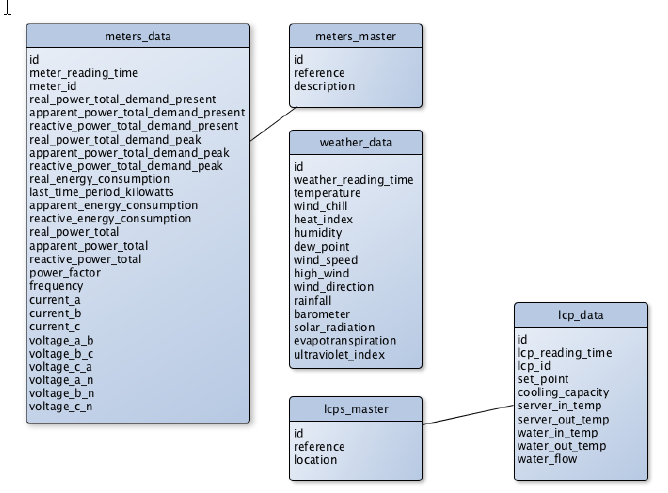
\includegraphics[scale=0.45]{TSSG_Data_Schema}

\end{figure}

 

As we see from the schema, the data captures a multitude of metered energy usage variables, different weather data, and water usage data. A full detailed definition of the key metrics is provided in the appendices - section \ref{sec:[Definition of key Variables]}. The data outlined here is available from 2014 right up to present, captured at 5 minute intervals, making this a time series data set. In the next section, the data is explored at an initial level to find any seasonal trends or predictive variables.
 
\subsection{Exploratory Data Analysis}
\label{subsec:[Exploratory Data Analysis]}
The data analysed for this project is a static 'data dump'. Additional data, when available, can be added for future studies if required. The data was accessed by connecting remotely into the Data Centre via PuTTY and querying the data via MySQL (See Appendices - section \ref{sec:[MySQL Queries]}). From here, the CSV output from the SQL queries was SFTP'd to my local machine and exported into Microsoft Excel where some preliminary data analysis was carried out. 

The schema introduced in Figure \ref{fig:TSSGdataschema} outlines the vast scale of variables available and as such data is gathered in 5 minute intervals over four years, the amount of data accumulated is vast and can be challenging to work with. While Python is used for developing the Data Mining Techniques (see sections \ref{subsec:[Data Mining Techniques]} and \ref{sec:[Python Code]}) line charts are ideal to illustrate at an exploratory level, what the time series data can show and the following charts are snippets from the data to demonstrate the range of data available.

\begin{figure}[H]
  \caption{Energy consumption (in kW usage per 5 minute intervals) of one cabinet in the Data Centre over the entire year of 2017.}
  \label{fig:Annualenergyfigure}
  \centering
    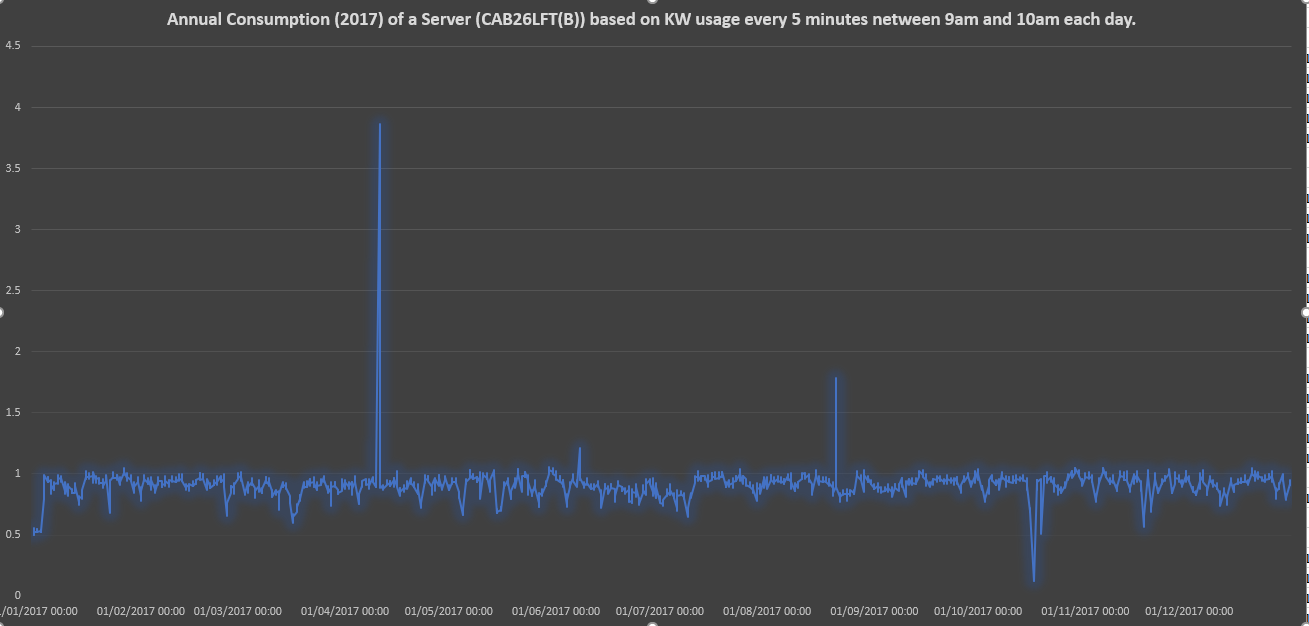
\includegraphics[scale=0.30]{Annual_energy_consumption}
\end{figure}

Figure \ref{fig:Annualenergyfigure}, generated using Listing~\ref{list:[Annual Energy Consumption]}, illustrates the energy consumption of one particular server cabinet within the Data Centre (Cabinet 26A) over the course of 2017. The daily readings are taken from between 9am and 10am each day and while the chart may initially suggest that the energy usage has been relatively consistent, there are significant spikes in energy consumption in April and August, with some considerable drops in demand too. 

However, while Figure \ref{fig:Annualenergyfigure} was a snapshot of energy usage over a year, the data can also be presented for a particular day. 

\begin{figure}[H]
  \caption{Energy consumption (in kW usage per 5 minute intervals) of three different server cabinets in the Data Centre over the course of one day (2017-09-13).}
  \label{fig:Dailyenergyfigure}
  \centering
    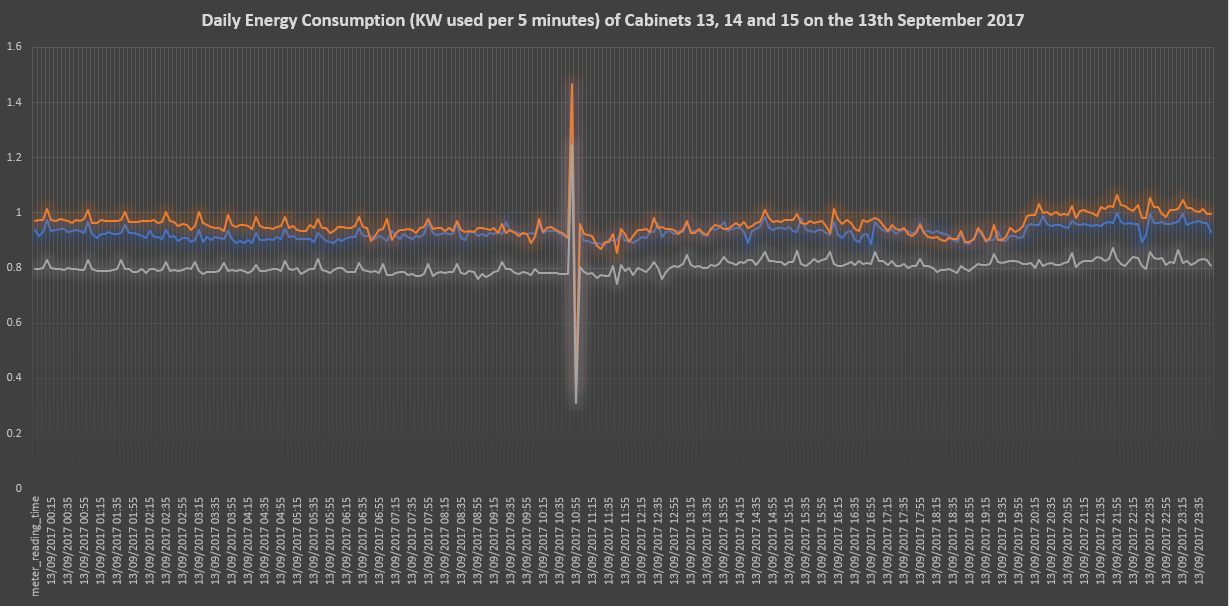
\includegraphics[scale=0.35]{Daily_energy_consumption_of_cab131415}
\end{figure}
   
Figure \ref{fig:Dailyenergyfigure} reports significant spikes in energy consumption in two of the cabinets around 11am. Again, this is another example of how Data Mining techniques might be applied to assist in being able to predict when such spikes occur. 

While certain spikes in energy consumption is suitable for further investigation, the preliminary data analysis should be able to detect some seasonal behaviour. Figure \ref{fig:cabvchillerfigure} demonstrates this. While the energy usage for the server cabinet (cabinet 26b) is relatively stable throughout the year, the energy consumption for the chillers shows a clear increase throughout the warmer summer months. Interestingly however, while each chiller works on alternate weeks, there are unexplained spikes for chiller B throughout the second half of the year that are not replicated when chiller A is running. 

\begin{figure}[H]
  \caption{Energy consumption (in kW usage per 5 minute intervals) of both Chillers and one server cabinet in the Data Centre over the course of 2017}
  \label{fig:cabvchillerfigure}
  \centering
    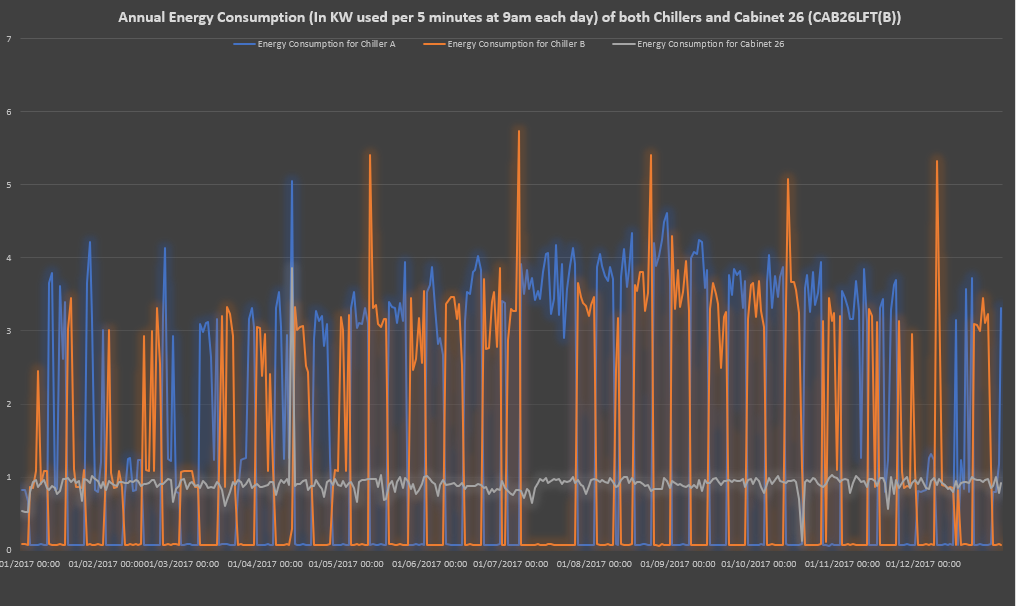
\includegraphics[scale=0.45]{Energy_consumption_of_cab26_and_chillers}
\end{figure} 

It is from presenting this information to Data Administrators who work in the Data Centre, where the impetus came to specifically concentrate on the inefficiency of the chiller system. It was their 'hunch' that such inefficiencies existed, and it was these discussions that spawned the third research question (in section \ref{subsec:[Research Questions]}).   

Other interesting preliminary analysis of the data centred around water consumption at the Data Centre (Figure \ref{fig:annualwaterfigure} ) and the energy usage of the generator during a severe weather event, in this case being Storm Ophelia on October 2017 (Figure \ref{fig:opheliafigure}). 

\begin{figure}[H]
  \caption{Annual water flow (in litres per 5 minute intervals) to LCP 1 measured at 9am every day during 2017}
  \label{fig:annualwaterfigure}
  \centering
    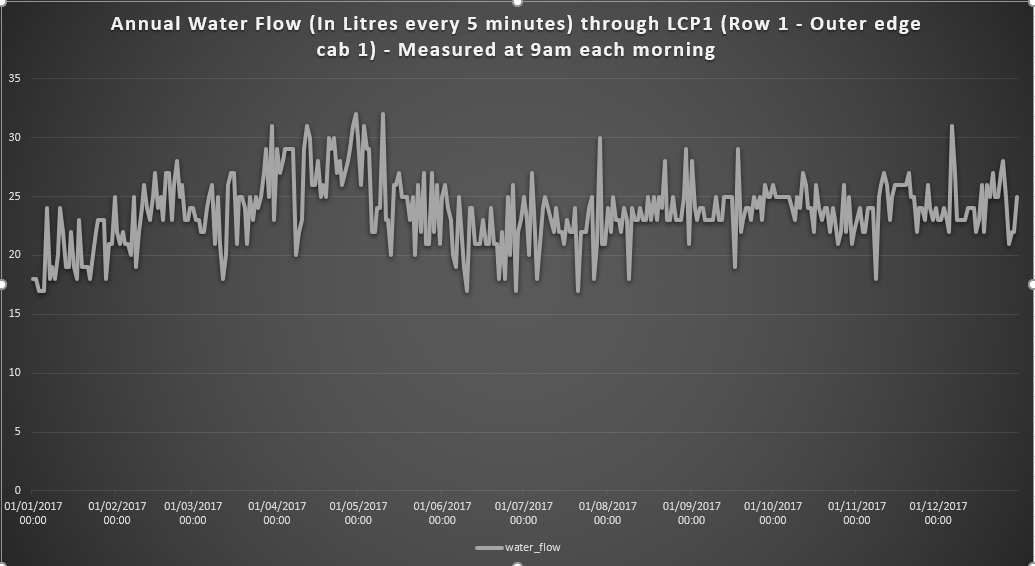
\includegraphics[scale=0.45]{Annual_Water_Flow}
\end{figure} 

\begin{figure}[H]
  \caption{Energy consumption (in kW usage per 5 minute intervals) of the Generator before, during and after Storm Ophelia in October 15th 2017}
  \label{fig:opheliafigure}
  \centering
    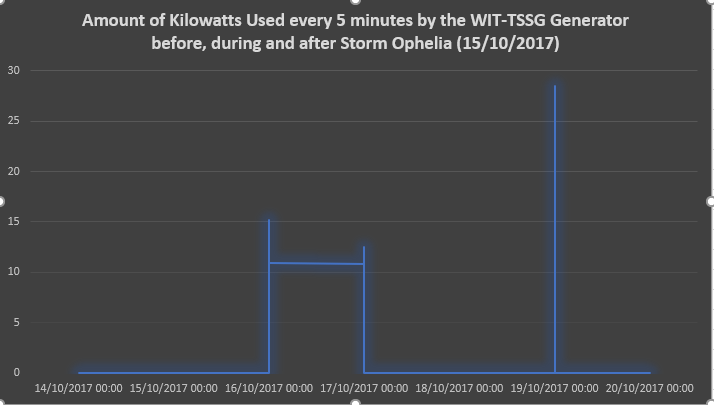
\includegraphics[scale=0.50]{Ophelia_generator}
\end{figure} 

All these charts are provided to simply demonstrate the range of data available. The next section discusses how this data was screened to build a model and the challenges that arose from this.  

\subsection{Research Techniques}
\label{subsec:[Research Techniques]}

\subsubsection{Introduction}
\label{subsubsec:[Introduction]}

An advantage for this research is that the data required is already available for analysis and the previous sections (\ref{subsec:[Data Available]} and \ref{subsec:[Exploratory Data Analysis]}) introduced the variables and did some exploratory data analysis. This section progresses further, and outlines how the data will be screened to build a model as outlined in the Methodology (section \ref{sec:[Methodology]}). 

Figure's \ref{fig:Annualenergyfigure}, \ref{fig:Dailyenergyfigure}, \ref{fig:cabvchillerfigure}, \ref{fig:annualwaterfigure} and \ref{fig:opheliafigure} demonstrate that the data available here is time series data. With data going back to 2014. This allowed for investigations into the energy usage per cabinet, per rack or even at a system level, whether that is the energy consumed by the network configuration, the server demand or other computational needs. 

The Exploratory Data Analysis section (\ref{subsec:[Exploratory Data Analysis]}) also illustrated seasonal effects where energy demand will increase in the summer months of the year as the warm weather precipitates the need for greater cooling within a Data Centre. However, the approach here will be to analyse these factors at a deeper level to build a more developed  model that unlocks hidden insights not yet discovered.

Firstly, the literature was reviewed from section \ref{subsec:[Data Mining Techniques]} and the various Data Mining techniques that have been used to increase energy efficiency of different building and heating systems taken into consideration. After this, the data was imported into Python for detailed Data Mining exploration to generate the correlations among all variables. The output from this is outlined in section \ref{subsubsec:[Analyse Correlations]}. This was presented to Data Administrators in the Data Centre who provided context to these findings and suggested specific areas to investigate.   %Some of these are utilised here to identify predictive variables and build a predictive model (section \ref{subsubsec:[Construct Predictive Model]}).

From here, regression analysis will look at the relationship between the performance of both Chillers with other variables. However, a model is only useful if it's reliable, meaning it should be accurate and precise. In attempting to develop such a model it will be important to focus on goodness of fit measures like bias, variance and auto-correlation. This will be a key factor in the project also.

Finally, as outlined in section \ref{subsec:[Data Available]}, it is important to note that the data presented here is a static 'data dump'. This allows for the development of models on the static data only. However, an advantage of having nearly five years of static data is that it allows for the model to be tested on different subsections of the data to test its validity and reliability.  Therefore data from 2017 has been used in the analysis so far. While this is useful and would solve for our research questions (section \ref{subsec:[Research Questions]}) concerning increasing energy efficiency within a Data Centre, a more ideal model would be based on live streaming data. This would allow us to solve for problems outlined in real-time and develop models that will assist in anomaly detection or highlight when system failures might occur in real time and assist in avoiding such failures. 

\subsubsection{Import Data From Data Centre}
\label{subsubsec:[Import Data From Data Centre]}

The first step was to retrieve the monitoring data for 2017 that is stored on the server of the Data Centre. Similar to the section \ref{subsec:[Exploratory Data Analysis]}, data was exported from the Data Centre by logging on remotely via PuTTY and directly querying the data, using MySQL (See Appendices - section \ref{sec:[Detailed MySQL Queries]}) and SFTP'ing the query results, as csv files, to my own local machine. 

Figure \ref{fig:TSSGdataschema}, as previously outlined, visualises what data is available in the Data Centre. Specifically, data from 2017 was used as an initial testing sandbox for the data analysis. As the time series data is gathered in 5 minute intervals, this equates to 175,200 entries for the entire year. 

In addition, specific monitoring data containing energy information from all 83 meter locations, \gls{LCP} information for all 15 \gls{LCP} locations and all weather variables were exported from the Data Centre. In total, for just 2017, that equated to over 210 million unique data entries, stored on three different csv files. 

\subsubsection{Understanding the Data}
\label{subsubsec:[Understanding the Data]}

With such a vast array of information available, as earlier demonstrated in section \ref{subsec:[Exploratory Data Analysis]}, the next stage was to streamline the amount of variables to be considered. After consultation, the following variables, as outlined in Figure \ref{fig:finalvariables}, were chosen.  

\begin{figure}[H]
  \caption{Schema of Data and Variables chosen for detailed Data Analysis}
  \label{fig:finalvariables}
  \centering
    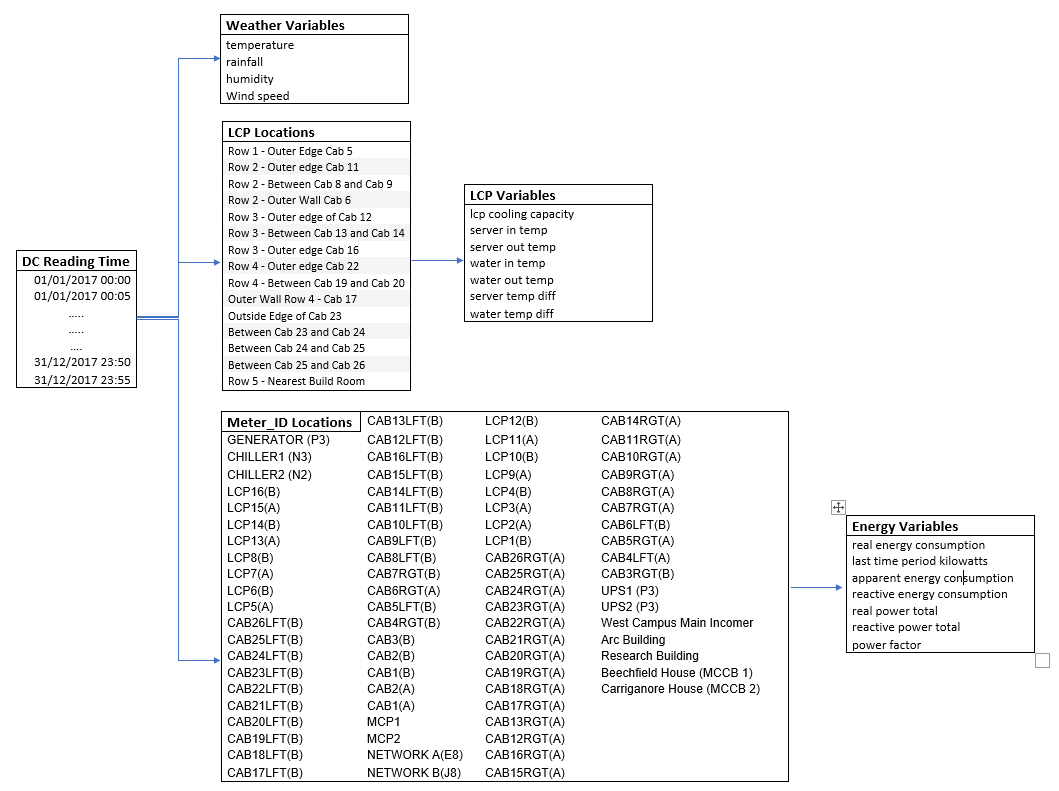
\includegraphics[scale=0.40]{finalvariables}
\end{figure} 

While full definitions of the key variables are defined in the appendices - section \ref{sec:[Definition of key Variables]} , the following diagram (Figure \ref{fig:coffeeenergyanaliogy}) describes and outlines the relationship between Real Power, Reactive Power, Apparent Power and Power Factor. 
%The following diagram briefly describes and outlines the relationship between \gls{Real}, \gls{Reactive}, \gls{Apparent} and \gls{Power}, while a full definition of these variables is available in the glossary.

\begin{figure}[H]
  \caption{The Latte Definition of Different Energy Metrics}
  \label{fig:coffeeenergyanaliogy}
  \centering
    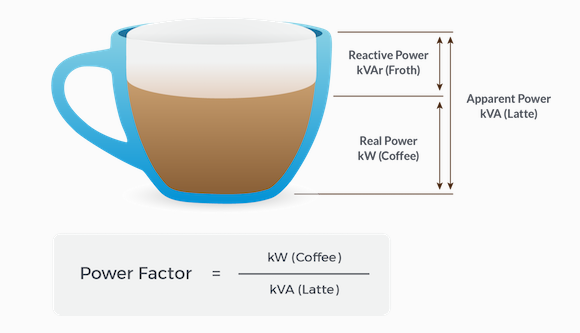
\includegraphics[scale=0.50]{power_explanation}
\end{figure} 

\subsubsection{Manipulate Data in Python to Generate Correlations for all Variables}
\label{subsubsec:[Manipulate Data in Python to Generate Correlations for all Variables]}

While a key requirement, as identified and prioritised during the project, was to focus on the Chiller system, it was also important to take a holistic view and unlock some insights about the Data Centre as a whole. Therefore, with the data now gathered, and the key variables identified, the next stage was to use Python to create correlations between all variables to identify some predictive features or new insights. The following steps were carried out in Python and the full code is viewable in section \ref{sec:[Python Code]} of the appendices.

\begin{enumerate}
\item Import csv's to Python.
\item Streamline data to only include selected variables. 
\item Use Pivot Tables to generate data based on the DC Reading time for every location and associated variable. 
\item Merge all energy, \gls{LCP} and weather information together to create a master table of all data based on the 5 minute interval values (merged on DC Reading Time).
\item Generate correlations based on the created time series for all 690 variables.
\item This created nearly 240,000 correlations. From this Python was Instructed to export the top 45,000 correlations for further analysis.
\end{enumerate} 

Ideally, during this process efforts would be made to reduce the dimensionality of the data so that further Python based analysis could take place such as heat maps. Unfortunately, any efforts with such an array of data was not possible due to computational limitations and while further attempts to do this later in the process was pursued, at this time it was deemed that it was more important to explore the all variables identified.

\subsubsection{Analyse Correlations}
\label{subsubsec:[Analyse Correlations]}

As Correlation analysis is the process to establish a relationship between two variables, the process to identify 'interesting' or 'useful' correlations in this instance was manual. Having received the top 45,000 correlations from Python, which had a correlation coefficient higher than +/- 0.93, this manual piece was done by importing the correlations to Microsoft Excel and using filters to trial and error different combinations. 

Some correlations between variables were easily explained, such as the relationship between different energy variables but the following are high-level findings from this process:    

\begin{itemize}
\item There is a strong correlation between Humidity (but not temperature) and \gls{Real}, \Gls{Apparent} and \Gls{Reactive}.
\item There is a high correlation between \Gls{Apparent} and \Gls{Real}. This indicates that there is a relatively stable amount of reactive power generated at each meter.
\item There is a high amount of correlation between Real power total and Last time kw.
\item In terms of analysing the different performances of the chillers, out of 2103 correlations, 2089 are identical for both Chiller 1 and Chiller 2. The main difference centres around some correlations for Chiller 2 and the \gls{LCP} and server temp differences of some cabinets.
\item In terms of cross-correlations between meter id’s and LCP locations, there is a high correlation between \Gls{Real} of most meter id’s and 5 particular \gls{LCP} variables that is very consistent.
\end{itemize}  

Full details of the correlation analysis, including a definition of the key variables discussed are found in section \ref{sec:[Data Centre Correlation Analysis Results]}. 

\subsubsection{Meet with Data Centre Administrators}
\label{subsubsec:[Meet with Data Centre Administrators]}

Various meetings with Data Centre Administrators took place during this process. These ranged from tours of the Data Centre, to in-depth discussions around possible areas of investigation and also detailed discussions around preliminary findings. 

In particular, they highlighted the inefficiencies in the Chiller system. Specifically, they explained how the two chillers alternate weeks in operation and how chiller 1 uses considerably more energy when it kicks in for its rotation.

It's from these meetings, that the third research question around the energy inefficiency of the chiller system got initially prioritised. The Data Administrators have a cost incentive to correctly identify the issue at stake, so that the specific hardware component can be replaced in isolation. Because without precisely identifying the component at fault, the cost of repairing the system increases exponentially. 

Therefore, from the Data Administrator's perspective their stated priority is to investigate the issues around the chiller system more so than predicting energy demand. Therefore, that's why the focus for this work narrows from here to look at the Chiller system. A predictive model is still constructed but is used in the context of comparing the performance of both chillers. 

%However, as explained in the research questions (section \ref{subsec:[Research Questions]}, to prioritise this stream of work will require hands-on participation from the Data Administrators through to the end of the project. This is because of their technical knowledge of the electrical and plumbing systems associated with the chiller system. They also have access to further data around the water pressure within the system that is not available to me currently. So for this stream of work to reach a successful conclusion, the Data Administrators need to become partners in the research, not just consultants. At this stage, without this being confirmed, the third research question is only under consideration at this time, with the situation being actively managed in the short term to balance the overall priorities of the project.  


\subsubsection{Identify Micro-timelines to Analyse Chiller Performance}
\label{subsubsec:[Identify Micro-timelines to Analyse Chiller Performance]}

Section \ref{subsubsec:[Analyse Correlations]} investigated correlations between all variables over the course of a year. However, that timescale is too broad to draw definitive conclusions about the performance of the Chiller system. Therefore, we need to discover specific windows throughout the year where there was visible anomalies in the performance of Chiller 1, and analyse those in isolation. To do this, the Apparent Power of both Chillers were charted on a line graph for the entire year to identify any such spikes. 

\begin{figure}[h]
  \caption{Apparent Energy Consumption of Chiller 1 and 2 in 2017}
  \label{fig:energyconsumptionchiller12}
  \centering
    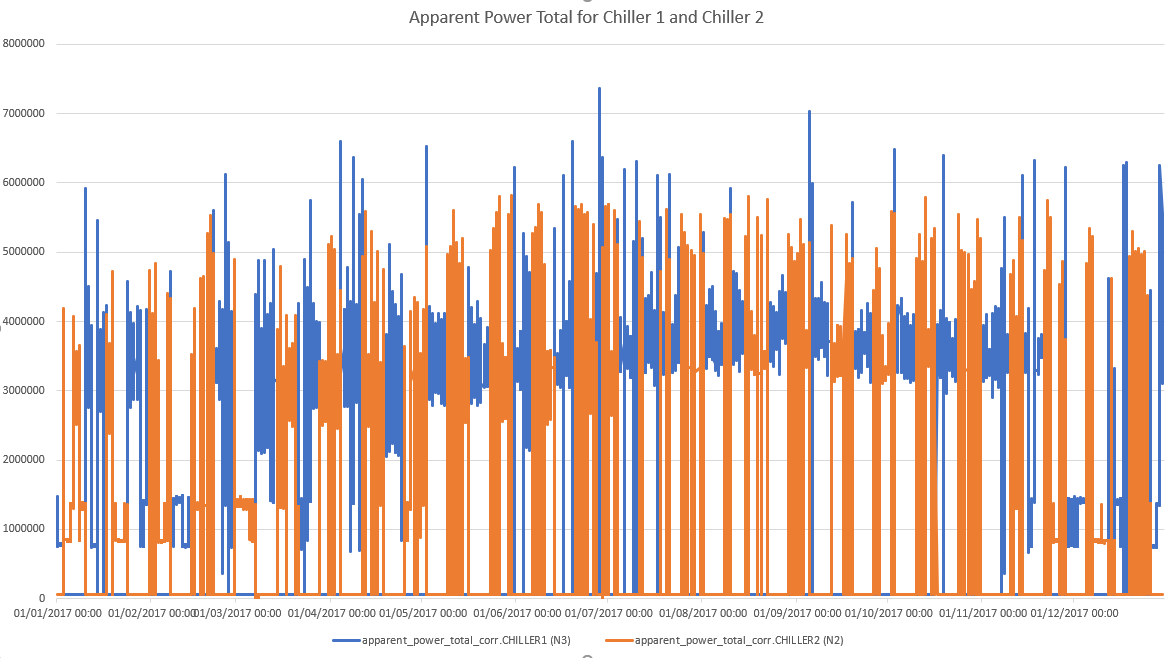
\includegraphics[scale=0.50]{energyconsumptionchiller12}
\end{figure} 

The diagram clearly illustrates many spikes (in blue) that have no corresponding orange spike, highlighting the prevalence of energy consumption spiking for Chiller 1. In particular, the following cutover dates, when the chiller alternated from Chiller 2 to Chiller 1, were identified for further analysis. 
\begin{enumerate}
  \item 2nd May 2017
   \item 13th June 2017
  \item 5th September 2017 
\end{enumerate}

The next step is to take the week before the cutover, and the week after the cutover to analyse the correlations between the chiller in operation for that week, and the other variables. In theory they should be relatively stable, so any correlations that are present in one week and not the subsequent week indicates a potential issue. 

\subsubsection{Identifying Variables to use in a Regression Model}
\label{subsubsec:[Identifying Variables to use in a Regression Model]}

Ultimately, with 690 variables potentially available, a process was needed to identify some key variables to use in a regression model to analyse the performance of both Chillers. This was done by using correlation analysis, similar to section \ref{subsubsec:[Analyse Correlations]}. However, the key difference was that this analysis was focused on just a particular week and that the correlations were focused around just the Chiller in operation for that week. The following steps were carried out in Python and the full code was similar to that as referenced in section \ref{sec:[Python Code]} of the appendices, with minor filters applied for date ranges and specific variables.

\begin{enumerate}
\item Import saved data from previous Python code where all data is merged and ready for use (Section \ref{subsubsec:[Manipulate Data in Python to Generate Correlations for all Variables]})
\item Streamline data to only include data from the week before the Cut-over (25th April to 2nd May)  
\item Generate correlations based on the created time series for all 690 variables.
\item This created nearly 240,000 correlations. From this Python was Instructed to export the top 30,000 correlations for further analysis.
\item Streamline data to only include data from the week after the Cut-over (2nd May to 9th May) 
\item Generate correlations based on the created time series for all 690 variables.
\item This created nearly 240,000 correlations. From this Python was Instructed to export the top 30,000 correlations for further analysis.
\item Repeat this step for the other 2 cut-over times identified.
\end{enumerate}  

This provided 2 sets of correlations for each Micro-timeline, the first for Chiller 2 and the second for Chiller 1. These were exported to excel and were manually compared to to identify, for each Micro-timeline, significant differences in correlation co-coefficients between the same variables. As the Correlation co-coefficients should be consistent from week to week, any particular variables that were not similar between both weeks were earmarked to be used in the regression model.

An overview of the outcome of this process is outlined in the Presentation of Findings (section \ref{sec:[Presentation of Findings]}) and the full detailed results are in the Appendices section \ref{sec:[Chiller Correlation Analysis Results]}. 

In selecting variables for the regression model, the four weather variables were included to control for external factors, while the remaining 40 variables were identified using the correlation analysis in this section. As there are several energy consumption metrics, Apparent Power was used to bring consistency to the model.       


\subsubsection{Construct Regression Model}
\label{subsubsec:[Construct Regression Model]}

As per sections \ref{subsec:[Research Questions]} and \ref{sec:[Methodology]}, the aim is to construct a regression model around the energy consumption of the Chiller in operation for that week \textit{(dependent variable)} with selected other variables, identified in section \ref{subsubsec:[Identifying Variables to use in a Regression Model]}, such as the weather, energy consumption of certain cabinets and specific water cooling features \textit{(independent variables)}. 

\begin{equation}
\hat{Y}_i = \hat{\beta}_0 + \hat{\beta}_1 X_i + \hat{\epsilon}_i
\end{equation}

The full variable list of Independent Variables used is available in the Appendices - section \ref{sec:[Full list of Independent Variables for Regression Model]}. We then compare the coefficients of this model, taking the confidence intervals into account, to the same results the next week, when the alternating Chiller is in operation. 

The premise of this model is that over a two week period, the relationship of the independent variables to the Chiller in operation for each week, as measured by the model, should be relatively stable. Independent variables therefore, that are not stable from week to week, especially those are also present in analysing the other cut-over times, indicate potential issues with how the Chillers operate and possible inefficiencies in how the Data Centre manages its supply of electricity. This is how this model proposes to answer the Research Questions as outlined in section \ref{subsec:[Research Questions]}.  


\subsubsection{'Goodness of Fit' Measures}
\label{subsubsec:['Goodness of Fit' Measures]}
However, there are a number of 'Goodness of Fit' factors to consider when constructing the regression model. As this is time series data, the data needs to be stationary, meaning that statistical properties such as \textit{mean} and \textit{variance} are constant over time. The Augmented Dickey-Fuller Test was used to confirm that the time series was stationary.

In addition, the model also needed to be conscious of \textit{Auto-Correlation}. This is to check that the similarities between variables is not as a result of a time-lag between them. The Durbin-Watson statistic from the regression output quantifies this test. The result is a score between \textit{0} and \textit{4}, with anything between \textit{0} and \textit{2} indicating strong positive auto-correlation and between \textit{2} and \textit{4} indicating strong negative auto-correlation. Ideally a regression model would have a score close to \textit{2} which indicates no auto-correlation. However, the simple linear model as described in section \ref{subsubsec:[Construct Regression Model]} indicated strong auto-correlation in all six outputs of the model (for each week before and after a cut-over  for the 3 cut-over times being analysed). This meant that residual coefficients would be biased for each output so they could not be compared week to week.      

To overcome this, the Cochrane-Orcutt procedure was used which adjusts a linear model for auto-correlation in the error term. Once this was applied, and the model re-run, the 6 outputs of the regression model all scored a Durbin Watson score close to \textit{2}. 

This allowed for the comparison of residual coefficients from week 1 and week 2, for the three micro-timelines outlined and to identify the independent variables that are causing potential energy inefficiencies. 

Python was used to construct and execute the regression model and goodness of fit measures, and this code is captured in the Appendices - section \ref{sec:[Python Code for Regression Model]}. 

The results of the regression analysis are presented in the next section (\ref{sec:[Presentation of Findings]}) and discussed in section \ref{sec:[Discussion of Findings]}.   


\section{Presentation of Findings}
\label{sec:[Presentation of Findings]}

\subsection{Correlation Analysis of Chiller 1 versus Chiller 2}
\label{subsec:[Correlation Analysis of Chiller 1 versus Chiller 2]}

The process, which analysed the Correlation of the energy consumption of an active Chiller during the week before and after a cut-over with other variables is outlined in section \ref{subsubsec:[Identifying Variables to use in a Regression Model]} and the full detailed results are in the Appendix - section \ref{sec:[Chiller Correlation Analysis Results]}. The Python code for manipulating the data and generating the relevant correlations is in the Appendices - section \ref{sec:[Python Code]}. 

In Summary, for the first instance investigated, which covered the timeframe of April 25th through to May 9th, with the cut-over to Chiller 1 on May 2nd, out of 1,400 correlations relating to both Chillers, over 1,200 correlation coefficients match from week 1 to week 2. Out of the correlations that were not present in both weeks, The Energy Consumption of Cabinets 1, 7 and LCP units 5 and 19 along with Humidity were correlated with Chiller 2 only, while The Energy Consumption of Cabinets 3, 17 and LCP unit 7 were correlated only with Chiller 1. Interestingly, Chiller 1 was also only correlated with Water Flow and Server Temperature metrics between Cabinets 13 and 14.

Similarly, for the second instance investigated, which covered the timeframe of June 6th through to June 20th, with the cut-over to Chiller 1 on June 13th, out of 2,300 correlations relating to both Chillers, over 1,200 correlation coefficients match from week 1 to week 2. Out of the correlations that were not present in both weeks, The Energy Consumption of Cabinets 10, 22 and LCP units 9 and 17 along with LCP cooling metrics for Cabinet 22 were correlated with Chiller 2 only, while The Energy Consumption of Cabinets 3, 7, 12, 18 and LCP unit 7 were correlated only with Chiller 1. Again, Chiller 1 was also only correlated with Water Flow and Server Temperature metrics between Cabinets 13 and 14. 

Finally, for the final instance investigated, which covered the timeframe of August 29th through to September 12th, with the cut-over to Chiller 1 on September 5th, out of 1,700 correlations relating to both Chillers, over 1,250 correlation coefficients match from week 1 to week 2. Out of the correlations that were not present in both weeks, The Energy Consumption of Cabinets 22, 23, 24, 26 and LCP units 12 and 13 along with LCP cooling metrics for Cabinet 22, 23, 24 and 25 were correlated with Chiller 2 only, while The Energy Consumption of Cabinets 11 and the LCP units of 2, 5 and 11 were correlated only with Chiller 1. In addition, Chiller 1 was also only correlated with Water Temperature metrics between Cabinets 23 and 25 and Windspeed.   

The variables highlighted above, whose correlation coefficient with the energy consumption of the operating Chiller from week to week varied significantly after the cut-over in operating Chillers, potentially provides diagnostic information on features in the Data Centre where energy is being consumed inefficiently. These variables therefore form the basis of the regression model outlined in section \ref{subsubsec:[Construct Regression Model]}. The full list of variables used is outlined in the Appendices - section \ref{sec:[Full list of Independent Variables for Regression Model]}. 

\subsection{Regression Analysis of Chiller 1 versus Chiller 2}
\label{subsec:[Regression Analysis of Chiller 1 versus Chiller 2]}

In developing the model, the full process to construct the model and then to test that the time series is stationary is outlined in section \ref{subsubsec:[Construct Regression Model]}. It was confirmed that the time series was stationary. In all 6 instances of running the model, the Augmented Dickey-Fuller value is less than the 1\% critical value so we can reject the null hypothesis - confirming the presence of a stationary time series. 

In testing for Auto-correlation, whereas the original Linear regression models had a Durbin-Watson score of between \textit{0} and \textit{1}, confirming the presence of positive auto-correlation, which rendered the output biased. Using the Cochrane-Orcutt procedure to eliminate the bias, the generalised least squares method produced Durbin-Watson scores, for the 6 instances of the regression model of between \textit{1.89} and \textit{2.02}. As a score close to \textit{2} indicates no auto-correlation, the residual coefficients of each independent variable can be compared week to week, to identify where the relationship between the Chiller in operation and the independent variables differed significantly after the cut-over of the Chiller. 

This was done by matching the coefficients of the independent variables from week 1 to week 2, allowing for the \textit{0.025} and \textit{0.975} confidence intervals. This means that the coefficient value from week 1, would have to record a value between the confidence levels of the same variable for Week 2 and visa versa. The full breakdown, including the coefficient values for all 3 micro-timelines are in the Appendices - section \ref{sec:[Summary of the Output of the Regression Model]} while the Python code is also in the Appendices - section \ref{sec:[Python Code for Regression Model]}. A summary of the variables, whose coefficients do not match from week 1 to week 2, for the 3 micro-timelines is provided in Figure \ref{fig:regressionresults}.

\begin{figure}[H]
  \caption{Summary of Analysis from Regression Model}
  \label{fig:regressionresults}
  \centering
    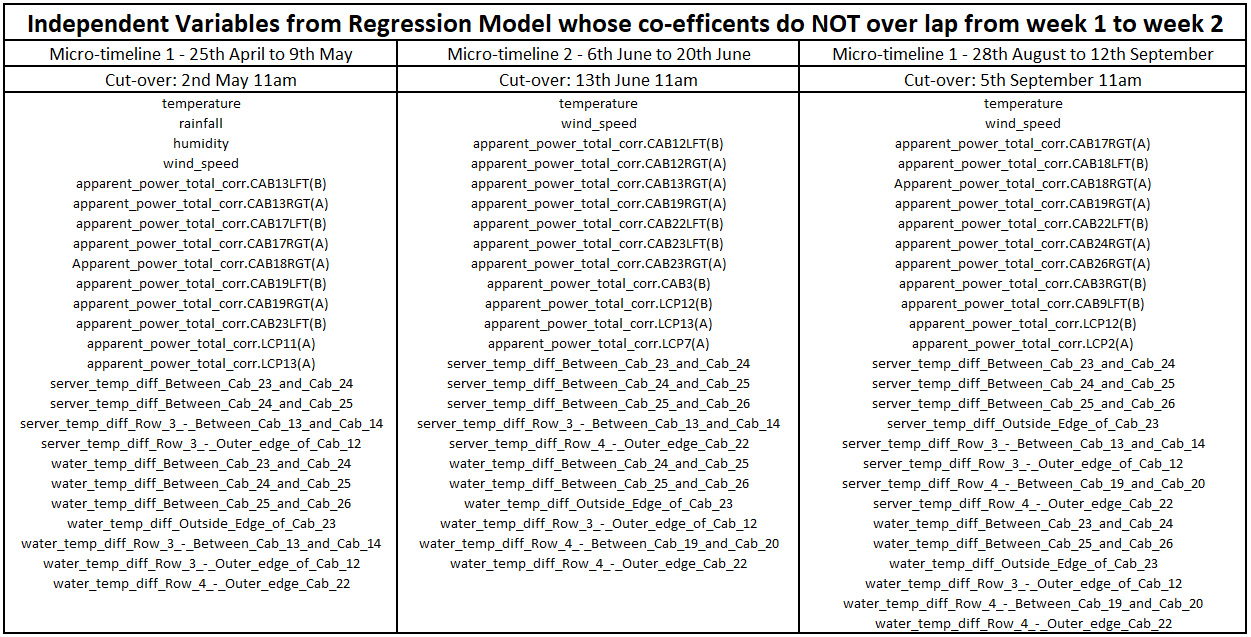
\includegraphics[scale=0.50]{regressionresults}
\end{figure}   

While the significance of these findings is discussed below in section \ref{sec:[Discussion of Findings]}, this highlights that while the majority of independent variables have a stable and consistent relationship to the dependent variable (the operational Chiller) from week 1 to week 2, the variables listed in Figure \ref{fig:regressionresults} do not. It is also worth noting that some variables are consistently present across multiple micro-timelines in Figure \ref{fig:regressionresults} which indicates the presence of a pattern.              

\section{Discussion of Findings}
\label{sec:[Discussion of Findings]}

From the outset, the exploratory data analysis (section \ref{subsec:[Exploratory Data Analysis]}) carried out on simple monitoring data, (Figures \ref{fig:cabvchillerfigure} and \ref{fig:energyconsumptionchiller12}) demonstrated that there was unexplained peaks in energy consumption of Chiller 1, which was further corroborated by staff working in the Data Centre. Therefore, the aim of this project as outlined in the Research Questions (section \ref{subsec:[Research Questions]}) and the Aims and Objectives (section \ref{subsec:[Aims and Objective]}) was to use monitoring data combined with Data Mining techniques to identify hidden insights as to why the Chiller system, and subsequently the Data Centre as a whole is consuming energy inefficiently. 

The correlation analysis, which looked at the Data Centre as a whole (section \ref{subsubsec:[Manipulate Data in Python to Generate Correlations for all Variables]}) and specifically for correlations between the operating Chiller and all other variables (section \ref{subsubsec:[Identifying Variables to use in a Regression Model]}) also provided some interesting findings. Specifically it emerged that energy consumption is more correlated with humidity than temperature.

That process also discovered variables that were not correlated to the same degree with the operational Chiller when the cut-over from Chiller 2 to Chiller 1 happened. These are interesting, as they are the exception with over 75\% of the variables recording a correlation coefficient that is stable and consistent across both weeks when the cut-over to Chiller 1 happens. Significantly again, some variables were present in the analysis across multiple micro-timelines indicating a potential underlying issue with their performance vis a vis the operating Chiller.     

However, as richer data is achieved from regression analysis, these variables then formed the basis for the regression model to quantify the relationship between the operating Chiller for a particular week and these selected other \textit{independent variables}. When the results for week 1 were compared with week 2, this again highlighted particular variables whose relationship to the operating Chiller was not consistent across both weeks. In analysing Figure \ref{fig:regressionresults}, there are some assumptions which must be stated. 

\begin{enumerate}
\item It would be expected that the 'weather' variables are not consistent from week 1 to week 2. This is Ireland after-all. These were included so that their relationship to the Chiller could still be measured (even if the weather varied wildly from week to week. 
\item The demand for energy consumption for any given cabinet \textit{could} vary from week to week also. It is not unforeseeable that a particular client of the Data Centre has differing requirements from week to week. To mitigate this, that's why data was gathered for a week prior to the cut-over and not just 2-3 days. However, if the same cabinet had a consistently different relationship to the operating Chiller from week to week it would be more alarming.    
\item The water and server temperature variables could be related to the weather. If the humidity raised considerably in week 2, that would have knock on effects on these variables. However, again, if they consistently had a different relationship to the operating Chiller from week 1 to week 2 it would raise alarm. The weather in Ireland doesn't fluctuate that much in such short spaces of time. Also to mitigate this the variable used in the model is water/server temperature difference. This is a contrived variable (developed in Python as demonstrated in the Appendices - section \ref{sec:[Python Code]}) to eliminate the fluctuations in the actual rise in the temperature and simply record the in/out difference in the temperature.  
\end{enumerate} 

Taking this into account, some inferences can still be drawn from the results as outlined in Figure \ref{fig:regressionresults}. The energy consumption of Cabinets 3, 12, 13, 17, 18, 22 and 23 as well as the LCP units of 12 and 13 appear on the list more than once. What this translates as is that more than once during our analysis, when the operating Chiller switched from Chiller 2 to Chiller 1, these cabinets and LCP units suddenly had a different relationship to the energy consumption of Chiller 1 than it had with Chiller 2. Furthermore, the energy consumption of Cabinet 19 has a different relationship to the operating Chiller across both weeks for all Micro-timelines. These results are also consistent with the correlation analysis of both Chillers. 

In addition, and maybe more significantly, the relationship between the operating chiller and the water temperature difference \textit{(the difference in water temperature entering and leaving the unit}) and server temperature difference \textit{(the difference in server temperature following the water being applied to cool the servers)} is far from stable from week to week. Particularly this is true of the cooling operations Between cabinets 23, 24, 25 and 26 an this is consistent over all 3 micro-timelines. What this indicates, is that when Chiller 1 cut-in to be the operating chiller, it had a consistently different relationship to these cooling variables than Chiller 2 did. Again, this was broadly consistent with the correlation analysis of both Chillers.        

In conclusion, while the analysis carried out here is consistent and highlights certain variables that may be responsible for inefficient energy consumption in the Chiller system, in terms of drawing definitive conclusions from the findings, that is not for me to say. I am not a field expert and all I can do is pass this information onto the Data Administrators and Engineers in the Data Centre for further analysis on their side. To add to this, this project, with all the constraints of a taught masters programme, only looked to use correlation and regression techniques on 3 micro-timelines to garner these results and findings. It has to be stated that there is much scope for further analysis using both extended Data Mining techniques and additional data. Richer data around water pressure was not made available in time for this project but does exist. This along with deeper analysis into other years could yield potentially richer results.   

However, to answer the 3 Research Questions as stated in section \ref{subsec:[Research Questions]}, a model was constructed, using monitoring data from a Data Centre and combining this with Data Mining techniques to identify hidden features which might find anomalies or inefficiencies in energy consumption. We identified that energy consumption of Chiller 1 spikes when it takes over from Chiller 2 on a weekly rotation, and the regression results here show a link to certain water and server temperature variables of specific cabinets when this happens.   These are the hidden features that are not evidently visible from normal monitoring data and this information will be passed to the relevant people in the Data Centre to fully understand these findings.     

\section{Conclusion}
\label{sec:[Conclusion]}
This project concentrates on the growing prevalence that Data Centres play in the ICT sector and how much energy they currently consume. The literature review introduces Data Centres in more detail, including the WIT-TSSG Data Centre, before surveying the existing literature that focused on increasing the energy efficiency of Data Centres.  The literature review also looks at how Data Mining Techniques are used in increasing energy efficiency of other building types before a gap was established where Data Mining techniques could be used to help Data Centres become more energy efficient. 

The Methodology section expanded on this gap and set the framework for the research methods section which firstly explains the data available before outlining the Data Mining techniques used to develop a model that will analyse the energy consumption of both Chillers. Specifically this model focused around when we see an an unexplained spike in the energy consumption of Chiller 1 and the model and subsequent analysis outlines potential features that may be responsible for such a spike in energy consumption. 

These results are presented and discussed with the caveat that it would require a Data Centre Engineer to interpret the findings fully and that there is much scope for further research to back up these findings. However, during the duration of finalising this document, it has been confirmed by staff in the Data Centre, that the Chiller system did indeed require remedial action and that is currently ongoing. Unfortunately at the time of completing this research it is too soon to say if the underlying physical issues uncovered acquiesce with my findings, but it does validate the decision to concentrate on energy inefficiencies in the Chiller system.       

Therefore in terms of the generalisability of this research, while all Data Centres will have similar monitoring data that consist of metered energy usage, weather information and other operational data, not all Data Centres will have the same geographical constraints or energy demands driven by its individual clients. So while there could be no direct inference made to other specific Data Centres, any findings could be relate-able in a broader sense if a common set of features or attributes can be found. This would be the contribution of this proposed study to the existing literature.    

Finally, in terms of the reasoning applied, this project with Data Mining at its core, straddles both inductive and deductive reasoning. When Data Mining is used in an exploratory mode, it is inductive while when it is used to build predictions, it is deductive. This project has elements of both as the quantitative data is already compiled and available (sections \ref{subsec:[Data Available]} and \ref{subsec:[Exploratory Data Analysis]}). It also exhibits abductive reasoning by finding an explanation for an apparent behaviour discovered in data. 

\newpage
\printbibliography[heading=bibintoc]
\newpage
\glsaddall
\printglossary
\newpage
\appendix
\appendixpage
\addappheadtotoc

\section{MySQL Queries for Exploratory Data Analysis}
\label{sec:[MySQL Queries]}
This section provides the MySQL queries used to source the data for the line charts in Figures \ref{fig:Annualenergyfigure}, \ref{fig:Dailyenergyfigure}, \ref{fig:cabvchillerfigure}, \ref{fig:annualwaterfigure} and \ref{fig:opheliafigure}.


\begin{listing}[H]
\begin{minted}{sql}
use dc; 
select * 
from meters_data
where meter_reading_time > '2017-01-01'
and meter_reading_time < '2017-12-31'
and HOUR(`meter_reading_time`) = 9
and meter_id not in ('1','2','3','4','5','6','7','8','9','10','11',
 '12','77','78');
\end{minted}
\caption{MySQL Query for Annual Energy Consumption}
\label{list:[Annual Energy Consumption]}
\end{listing}
%\end{lstlisting}

\begin{listing}[H]
\begin{minted}{sql}
use dc; 
select * 
from meters_data
where meter_reading_time > '2017-09-12'
and meter_reading_time < '2017-09-14'
where meter_id in ('13','14','15');
\end{minted}
\caption{MySQL Query for Daily Energy Consumption}
\label{list:[Annual Energy Consumption]}
\end{listing}

\begin{listing}[H]
\begin{minted}{sql}
use dc; 
select * 
from meters_data
where meter_reading_time > '2017-01-01'
and meter_reading_time < '2017-12-31'
and HOUR(`meter_reading_time`) = 9
and MINUTE(`meter_reading_time`) = 0
and meter_id in ('3','4','13');
\end{minted}
\caption{MySQL Query for Annual Energy Consumption of Chillers and Server}
\label{list:[MySQL Query for Annual Energy Consumption of Chillers and Server]}
\end{listing}

\begin{listing}[H]
\begin{minted}{sql}
use dc; 
select * 
from lcps_data
where lcp_reading_time > '2017-01-01'
and lcp_reading_time < '2017-12-31' 
and HOUR(`lcp_reading_time`) = 9
and MINUTE(`lcp_reading_time`) = 0;
\end{minted}
\caption{MySQL Query for Annual Water Flowr}
\label{list:[MySQL Query for Annual Water Flow]}
\end{listing}

\begin{listing}[H]
\begin{minted}{sql}
use dc; 
select * 
from meters_data
where meter_reading_time > '2017-10-10'
and meter_reading_time < '2017-10-24'
and meter_id = '2';
\end{minted}
\caption{MySQL Query for Energy Consumption of the Generator during Storm Ophelia}
\label{list:[MySQL Query for Energy Consumption of the Generator during Storm Ophelia]}
\end{listing}

\section{MySQL Queries for Detailed Data Analysis}
\label{sec:[Detailed MySQL Queries]}
This section provides the MySQL queries used to source the data for section \ref{subsubsec:[Import Data From Data Centre]}

\begin{listing}[H]
\begin{minted}{sql}
use dc; 
select * 
from meters_data
where meter_reading_time > '2017-01-01'
and meter_reading_time < '2017-12-31';
\end{minted}
\caption{MySQL Query for Energy Consumption in 2017}
\label{list:[MySQL Query for Energy Consumption in 2017]}
\end{listing}

\begin{listing}[H]
\begin{minted}{sql}
use dc; 
select * 
from meters_master;
\end{minted}
\caption{MySQL Query for All Meter ID Location}
\label{list:[MySQL Query for All Meter ID Location]}
\end{listing}

\begin{listing}[H]
\begin{minted}{sql}
use dc; 
select * 
from lcps_data
where lcp_reading_time > '2017-01-01'
and lcp_reading_time < '2017-12-31';
\end{minted}
\caption{MySQL Query for LCP information for 2017}
\label{list:[MySQL Query for LCP information for 2017]}
\end{listing}


\begin{listing}[H]
\begin{minted}{sql}
use dc; 
select * 
from lcps_master;
\end{minted}
\caption{MySQL Query for LCP Location Information}
\label{list:[MySQL Query for LCP Location Information]}
\end{listing}

\begin{listing}[H]
\begin{minted}{sql}
use dc; 
select * 
from weather_data
where weather_reading_time > '2017-01-01'
and weather_reading_time < '2017-12-31';
\end{minted}
\caption{MySQL Query for Weather Data for 2017}
\label{list:[MySQL Query for Weather Data for 2017]}
\end{listing}

\section{Python Code for Data Manipulation}
\label{sec:[Python Code]}
This section provides Python code to cleanse, manipulate and derive correlations the data in section \ref{subsubsec:[Analyse Correlations]}

%\begin{lstlisting}[frame=single,basicstyle=\footnotesize\ttfamily,
%  caption={Python - Set Up and Configuration},label={list:[Python - Set up and Configuration]}]
\begin{listing}[H]
\begin{minted}{python}
import numpy as np
import pandas as pd
pd.options.display.max_rows = 1000
import matplotlib.pyplot as plt
import seaborn as sns
sns.set_style("darkgrid")
sns.set_context("paper")
from itertools import combinations, groupby
from collections import Counter

import sys, os, glob
def size(obj):
"""Return size of object in MB"""
return "{0:.2f} MB".format(sys.getsizeof(obj) / (1000 * 1000))
\end{minted}
\caption{Python - Set Up and Configuration}
\label{list:[Python - Set up and Configuration]}
\end{listing}
%\end{lstlisting}

\begin{listing}[H]
\begin{minted}{python}
energyusagepython = pd.read_csv("data/energyusagepython.csv")

metersmaster = pd.read_csv("data/metersmaster.csv")

energy_info = energyusagepython.merge(metersmaster, on="meter_id")

energy_regression = energy_info[['meter_reading_time',
'description',
'real_energy_consumption',
'last_time_period_kilowatts',
'apparent_energy_consumption',
'reactive_energy_consumption',
'real_power_total',
'apparent_power_total',
'reactive_power_total',
'power_factor']]

energy_regression.columns = ['dc_reading_time','meter_location',
'real_energy_consumption',
'last_time_period_kilowatts',
'apparent_energy_consumption',
'reactive_energy_consumption',
'real_power_total',
'apparent_power_total',
'reactive_power_total',
'power_factor']

\end{minted}
\caption{Python - Import and Cleanse Energy Data}
\label{list:[Python - Import and Cleanse Energy Data]}
\end{listing}

\begin{listing}[H]
\begin{minted}{python}
last_time_period_kilowatts_corr = energy_regression.pivot_table
(index='dc_reading_time',
columns='meter_location',
values='last_time_period_kilowatts')

last_time_period_kilowatts_corr.columns =
 ['last_time_period_kilowatts.Arc Building',
  'last_time_period_kilowatts.Beechfield House (MCCB 1)',
  ........................
  'last_time_period_kilowatts.West Campus Main Incomer']
    
The same process was followed for all energy variables.

\end{minted}
\caption{Python - Pivot Data around the meter reading time}
\label{list:[Python - Pivot Data around the meter reading time]}
\end{listing}

\begin{listing}[H]
\begin{minted}{python}
last_time_period_kilowatts_corr.reset_index( inplace=True)
real_energy_consumption_corr.reset_index( inplace=True)
total_energy_info_1 = last_time_period_kilowatts_corr.merge
(real_energy_consumption_corr, on="dc_reading_time")

apparent_energy_consumption_corr.reset_index( inplace=True)
total_energy_info_2 = apparent_energy_consumption_corr.merge
(total_energy_info_1, on="dc_reading_time")

reactive_energy_consumption_corr.reset_index( inplace=True)
total_energy_info_3 = reactive_energy_consumption_corr.merge
(total_energy_info_2, on="dc_reading_time")

real_power_total_corr.reset_index( inplace=True)
total_energy_info_4 = real_power_total_corr.merge
(total_energy_info_3, on="dc_reading_time")

apparent_power_total_corr.reset_index( inplace=True)
total_energy_info_5 = apparent_power_total_corr.merge
(total_energy_info_4, on="dc_reading_time")

reactive_power_total_corr.reset_index( inplace=True)
total_energy_info_6 = reactive_power_total_corr.merge
(total_energy_info_5, on="dc_reading_time")

power_factor_corr.reset_index( inplace=True)
total_energy_info_final = power_factor_corr.merge
(total_energy_info_6, on="dc_reading_time")

\end{minted}
\caption{Python - Merge Energy Pivot Tables together}
\label{list:[Python - Merge Energy Pivot Tables together]}
\end{listing}

\begin{listing}[H]
\begin{minted}{python}
lcpdata2017 = pd.read_csv("data/lcpdata2017.csv")
print("lcpdata2017 -- dimensions: {0};   size: {1}".format
(lcpdata2017.shape, size(lcpdata2017)))

lcpdmaster = pd.read_csv("data/lcpdmaster.csv")

lcp_info = lcpdata2017.merge(lcpdmaster, on="lcp_id")

lcp_regression = lcp_info[['lcp_reading_time',
'location',
'cooling_capacity',
'server_in_temp',
'server_out_temp',
'water_in_temp',
'water_out_temp',
'water_flow']]

lcp_regression['server_temp_difference'] 
= lcp_regression['server_out_temp'] - 
lcp_regression['server_in_temp']
lcp_regression['water_temp_difference'] 
= lcp_regression['water_out_temp'] 
- lcp_regression['water_in_temp']

lcp_regression.columns = ['dc_reading_time',
'lcp_location',
'_lcp_cooling_capacity',
'server_in_temp',
'server_out_temp'
,'water_in_temp',
'water_out_temp',
'water_flow',
'server_temp_diff',
'water_temp_diff']

\end{minted}
\caption{Python - Import and Merge LCP Data}
\label{list:[Python - Import and Merge LCP Data]}
\end{listing}


\begin{listing}[H]
\begin{minted}{python}
_lcp_cooling_capacity = lcp_regression.pivot_table
(index='dc_reading_time',columns='lcp_location',values=
'_lcp_cooling_capacity')

_lcp_cooling_capacity.columns = 
['lcp_cooling_capacity_Row 1 - Outer edge Cab 1',
    'lcp_cooling_capacity_Row 1 - Outer edge Cab 5', 
    ........................
    'lcp_cooling_capacity_Row 5 - Nearest Build Room']
    
The same process was followed for all LCP variables.

\end{minted}
\caption{Python - Pivot Data around the LCP reading time}
\label{list:[Python - Pivot Data around the LCP reading time]}
\end{listing}

\begin{listing}[H]
\begin{minted}{python}
_lcp_cooling_capacity.reset_index( inplace=True)
server_in_temp.reset_index( inplace=True)
lcp_info_1 = _lcp_cooling_capacity.merge(server_in_temp, 
on="dc_reading_time")

server_out_temp.reset_index( inplace=True)
lcp_info_2 = server_out_temp.merge(lcp_info_1, 
on="dc_reading_time")

water_in_temp.reset_index( inplace=True)
lcp_info_3 = water_in_temp.merge(lcp_info_2, 
on="dc_reading_time")

water_out_temp.reset_index( inplace=True)
lcp_info_4 = water_out_temp.merge(lcp_info_3, 
on="dc_reading_time")

water_flow.reset_index( inplace=True)
lcp_info_5 = water_flow.merge(lcp_info_4, 
on="dc_reading_time")

server_temp_diff.reset_index( inplace=True)
lcp_info_6 = server_temp_diff.merge(lcp_info_5, 
on="dc_reading_time")

water_temp_diff.reset_index( inplace=True)
lcp_info_final = water_temp_diff.merge(lcp_info_6, 
on="dc_reading_time")

\end{minted}
\caption{Python - Merge LCP Pivot Tables together}
\label{list:[Python - Merge LCP Pivot Tables together]}
\end{listing}

\begin{listing}[H]
\begin{minted}{python}
weatherdata = pd.read_csv("data/weatherdata.csv")

weatherdata.columns = ['weather_id',
'dc_reading_time',
'temperature',
'wind_chill'
,'heat_index'
,'humidity'
,'dew_point'
,'wind_speed',
'high_wind',
'wind_direction',
'rainfall'
,'barometer',
'solar_radiation',
'evapotranspiration',
'ultraviolet_index']

revised_weatherdata = weatherdata[['dc_reading_time',
'temperature',
'rainfall',
'humidity',
'wind_speed']]


\end{minted}
\caption{Python - Import and Merge Weather Data}
\label{list:[Python - Import and Merge Weather Data]}
\end{listing}

\begin{listing}[H]
\begin{minted}{python}
final_data_merge_1 
= total_energy_info_final.merge
(lcp_info_final, on="dc_reading_time")

final_data 
= revised_weatherdata.merge
(final_data_merge_1, on="dc_reading_time")

final_data.to_csv("final_data.csv", 
index=False, header=True)


\end{minted}
\caption{Python - Merge all Data Together into one table}
\label{list:[Python - Merge all Data Together into one table]}
\end{listing}

\begin{listing}[H]
\begin{minted}{python}
final_data_correlations = final_data.corr()

final_data_correlations.to_csv
(\"final_data_correlations.csv\", 
index=False, header=True)


\end{minted}
\caption{Python - Get Correlations between all Variables}
\label{list:[Python - Get Correlations between all Variables]}
\end{listing}

\begin{listing}[H]
\begin{minted}{python}
def get_redundant_pairs(final_data_correlations):
    '''Get diagonal and lower triangular pairs of correlation matrix'''
    pairs_to_drop = set()
    cols = final_data_correlations.columns
    for i in range(0, final_data_correlations.shape[1]):
        for j in range(0, i+1):
            pairs_to_drop.add((cols[i], cols[j]))
    return pairs_to_drop
    
def get_top_abs_correlations(final_data_correlations, n=5):
    au_corr = final_data_correlations.corr().abs().unstack()
    labels_to_drop = get_redundant_pairs
    (final_data_correlations)
    au_corr = au_corr.drop
    (labels=labels_to_drop).
    sort_values(ascending=False)
    return au_corr[0:n]
    
Top_correlations = 
(get_top_abs_correlations
(final_data_correlations, 45000))

Top_correlations.to_csv
("Top_Correlation_45000.csv", 
index=True, header=True)


\end{minted}
\caption{Python - Analyse Correlations in Python}
\label{list:[Python - Analyse Correlations in Python]}
\end{listing}


\section{Python Code for Regression Model}
\label{sec:[Python Code for Regression Model]}
This section provides Python code to construct the regression model and goodness of fit measures as outlined in sections \ref{subsubsec:[Construct Regression Model]} and \ref{subsubsec:['Goodness of Fit' Measures]}

\begin{listing}[H]
\begin{minted}{python}
import numpy as np
import pandas as pd 
pd.options.display.max_rows = 1000
import matplotlib.pyplot as plt
import seaborn as sns
sns.set_style("darkgrid")
sns.set_context("paper")
from itertools import combinations, groupby
from collections import Counter
import scipy.stats as stats
import sys, os, glob
from pandas import Series
from statsmodels.tsa.stattools import adfuller
from sklearn import linear_model
import statsmodels.api as sm
import statsmodels.tsa.api as smt
from scipy.stats.stats import pearsonr
from scipy import stats
import statsmodels.formula.api as smf
import statsmodels.stats as sm_stats
from sklearn import linear_model

  def size(obj):
    """Return size of object in MB"""
    return "{0:.2f} MB".format(sys.getsizeof(obj) / (1000 * 1000))
\end{minted}
\caption{Python - Set Up and Configuration for Regression}
\label{list:[Python - Set up and Configuration for Regression]}
\end{listing}
%\end{lstlisting}

\begin{listing}[H]
\begin{minted}{python}
final_data = pd.read_csv("final_data_revised_2.csv")
print("final_data -- dimensions: {0};   size: {1}".format(final_data.shape, size(final_data)))
display(final_data.head())

final_data_revised = final_data[['dc_reading_time','temperature','rainfall','humidity','wind_speed',
    'apparent_power_total_corr.CAB10LFT(B)',
    'apparent_power_total_corr.CAB10RGT(A)',
    'apparent_power_total_corr.CAB12LFT(B)',
    'apparent_power_total_corr.CAB12RGT(A)',
    'apparent_power_total_corr.CAB13LFT(B)',
    'apparent_power_total_corr.CAB13RGT(A)',
    'apparent_power_total_corr.CAB17LFT(B)',
    'apparent_power_total_corr.CAB17RGT(A)',
    'apparent_power_total_corr.CAB18LFT(B)',
    'Apparent_power_total_corr.CAB18RGT(A)',
    'apparent_power_total_corr.CAB19LFT(B)',
    'apparent_power_total_corr.CAB19RGT(A)',
    'apparent_power_total_corr.CAB22LFT(B)',

	----------------------

    'server_temp_diff_Row 4 - Outer edge Cab 22',
    'water_temp_diff_Between Cab 23 and Cab 24',
    'water_temp_diff_Between Cab 24 and Cab 25',
    'water_temp_diff_Between Cab 25 and Cab 26',
    'water_temp_diff_Outside Edge of Cab 23',
    'water_temp_diff_Row 3 - Between Cab 13 and Cab 14',
    'water_temp_diff_Row 3 - Outer edge of Cab 12',
    'water_temp_diff_Row 4 - Between Cab 19 and Cab 20',
    'water_temp_diff_Row 4 - Outer edge Cab 22']]
display(final_data_revised.head())

\end{minted}
\caption{Python - Import and Manipulate data for Regression}
\label{list:[Python - Import and Manipulate data for Regression]}
\end{listing}
%\end{lstlisting}

\begin{listing}[H]
\begin{minted}{python}
Peak3_Week1 = final_data_revised[(final_data_revised['dc_reading_time'] > '2017-08-29 11:00:00') & (final_data_revised['dc_reading_time'] < '2017-09-05 11:00:00')]

Peak3_Week1.drop(['dc_reading_time'], axis=1, inplace=True)

Peak3_Week1.to_csv("Peak3_Week1.csv", index=True, header=True)

from pandas import Series
from statsmodels.tsa.stattools import adfuller
series = Series.from_csv('Peak3_Week1.csv', header=0)
X = series.values
result = adfuller(X)
print('ADF Statistic: %f' % result[0])
print('p-value: %f' % result[1])
print('Critical Values:')
for key, value in result[4].items():
	print('\t%s: %.3f' % (key, value))

\end{minted}
\caption{Python - Create Micro-Timeline and Check that Time Series is Stationary}
\label{list:[Python - Create Micro-Timeline and Check that Time Series is Stationary]}
\end{listing}

\begin{listing}[H]
\begin{minted}{python}
Peak3_Week1.drop(['apparent_power_total_corr.CHILLER1 (N3)'], axis=1, inplace=True)
y = Peak3_Week1['apparent_power_total_corr.CHILLER2 (N2)'].copy() 
X = Peak3_Week1.copy()
X.drop(['apparent_power_total_corr.CHILLER2 (N2)'], axis=1, inplace=True)

model = linear_model.LinearRegression()

X_constant = sm.add_constant(X)
lin_reg_Peak3_Week1 = sm.OLS(y,X_constant).fit()
lin_reg_Peak3_Week1.summary()

\end{minted}
\caption{Python - Construct Regression Model and Execute}
\label{list:[Python - Construct Regression Model and Execute]}
\end{listing}


\begin{listing}[H]
\begin{minted}{python}
acf = smt.graphics.plot_acf(lin_reg_Peak3_Week1.resid, lags=40 , alpha=0.05)
acf.show()

for column in X.columns:
    corr_test = pearsonr(X[column], lin_reg_Peak3_Week1.resid)
    print(f'Variable: {column} --- correlation: {corr_test[0]:.4f}, p-value: {corr_test[1]:.4f}')
    
X.apply(np.var, axis=0)

from scipy import stats

def normality_of_residuals_test(model):
    '''
    Function for drawing the normal QQ-plot of the residuals and running 4 statistical tests to 
    investigate the normality of residuals.
    
    Arg:
    * model - fitted OLS models from statsmodels
    '''
    sm.ProbPlot(model.resid).qqplot(line='s');
    plt.title('Q-Q plot');

    jb = stats.jarque_bera(model.resid)
    sw = stats.shapiro(model.resid)
    ad = stats.anderson(model.resid, dist='norm')
    ks = stats.kstest(model.resid, 'norm')
    
    print(f'Jarque-Bera test ---- statistic: {jb[0]:.4f}, p-value: {jb[1]}')
    print(f'Shapiro-Wilk test ---- statistic: {sw[0]:.4f}, p-value: {sw[1]:.4f}')
    print(f'Kolmogorov-Smirnov test ---- statistic: {ks.statistic:.4f}, p-value: {ks.pvalue:.4f}')
    print(f'Anderson-Darling test ---- statistic: {ad.statistic:.4f}, 5% critical value: {ad.critical_values[2]:.4f}')
    print('If the returned AD statistic is larger than the critical value, then for the 5% significance level, the null hypothesis that the data come from the Normal distribution should be rejected. ')
    
normality_of_residuals_test(lin_reg_Peak3_Week1)

\end{minted}
\caption{Python - Check Regression Model for Auto-Correlation and Other Tests}
\label{list:[Python - Check Regression Model for Auto-Correlation and Other Tests]}
\end{listing}


\begin{listing}[H]
\begin{minted}{python}
lin_reg_Peak3_Week1_CORC = smf.GLSAR(y,X)
lin_reg_Peak3_Week1_CORC_fit = lin_reg_Peak3_Week1_CORC.iterative_fit(maxiter = 100)
lin_reg_Peak3_Week1_CORC_fit.summary()

print(lin_reg_Peak3_Week1_CORC.rho) 

\end{minted}
\caption{Python - Run Cochrane-Orcutt Procedure (to eliminate autocorrelation)}
\label{list:[Python - Run Cochrane-Orcutt Procedure (to eliminate autocorrelation)]}
\end{listing}



\section{Definition of Key Variables}
\label{sec:[Definition of key Variables]}

This section provides definitions of key variables as discussed in section \ref{subsubsec:[Analyse Correlations]}

\begin{figure}[h]
  \caption{Definition of key Variables from the Monitoring Data}
  \label{fig:key_variables}
  \centering
    \includegraphics[scale=0.75]{"key_variables".png}
\end{figure} 



\section{Detailed Correlation Analysis Results for Overall Data Centre}
\label{sec:[Data Centre Correlation Analysis Results]}
This section provides the detailed correlation analysis as outlined in section \ref{subsubsec:[Analyse Correlations]}


\begin{figure}[H]
  \caption{The Detailed Correlation Analysis Results - section 1}
  \label{fig:Correlation_Analysis_1}
  \centering
    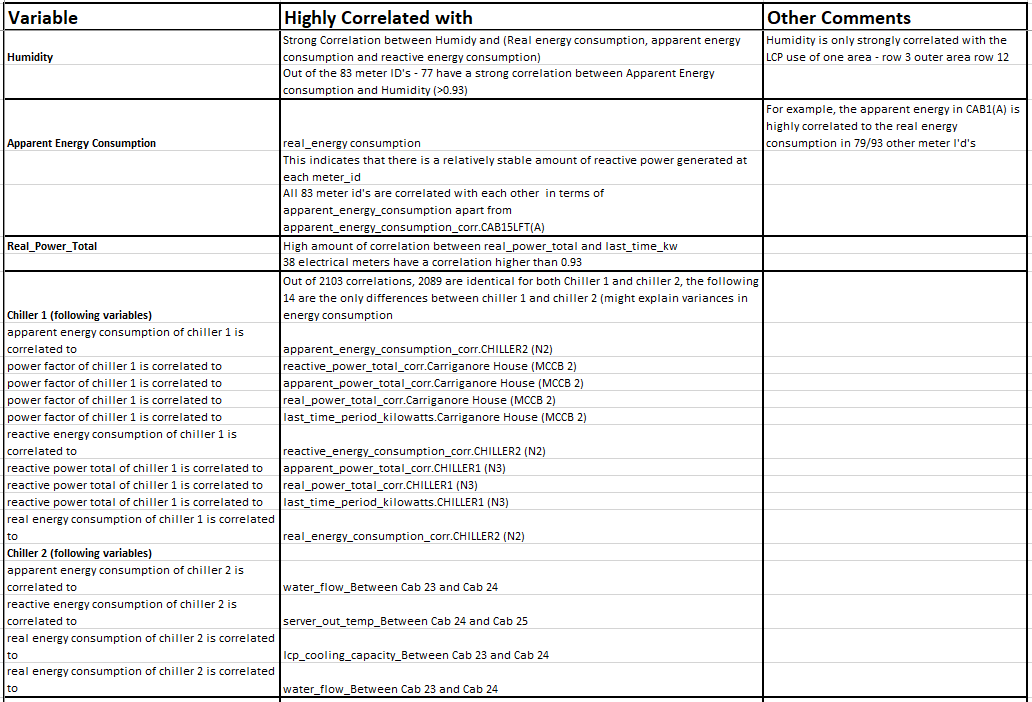
\includegraphics[scale=0.50]{Correlation_Analysis_1}
\end{figure} 

\begin{figure}[H]
  \caption{The Detailed Correlation Analysis Results - section 2}
  \label{fig:Correlation_Analysis_2}
  \centering
    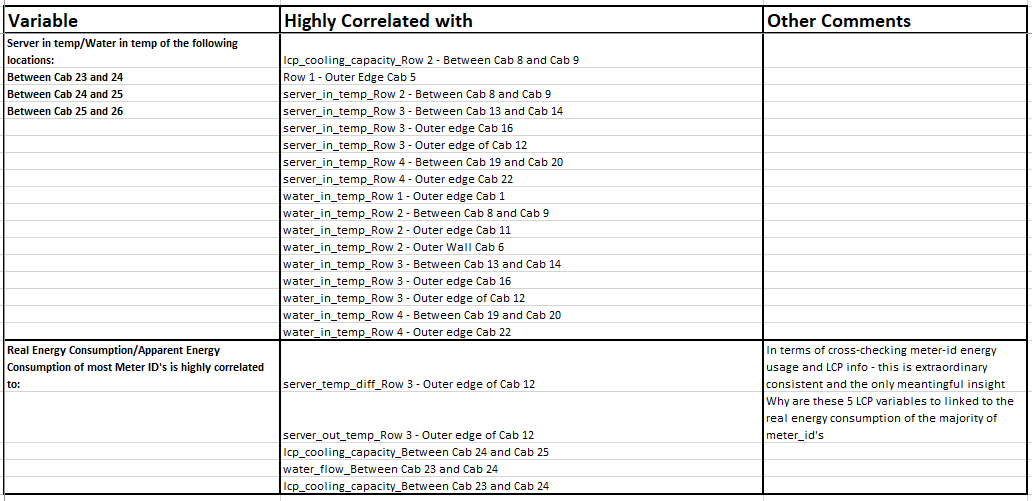
\includegraphics[scale=0.50]{Correlation_Analysis_2}
\end{figure} 

\section{Detailed Correlation Analysis Results for each Chiller}
\label{sec:[Chiller Correlation Analysis Results]}

\begin{figure}[H]
  \caption{Correlation Analysis of each Chiller for 4/28 to 5/9}
  \label{fig:peak1chillercorrelation}
  \centering
    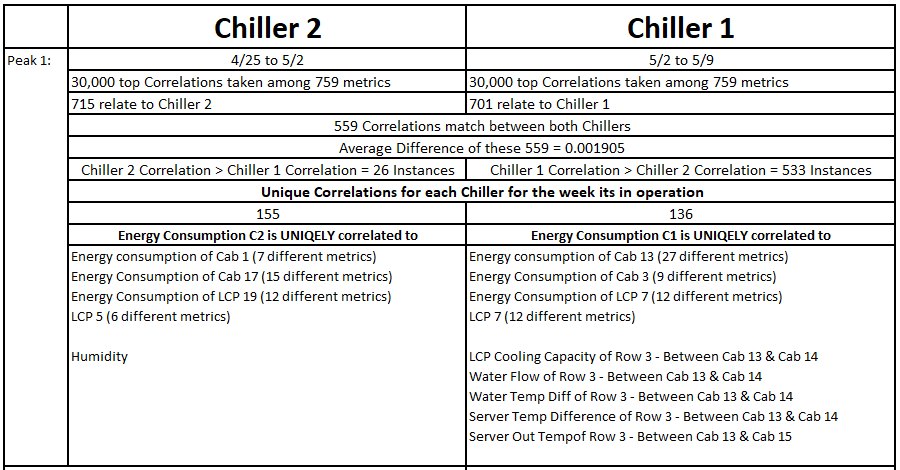
\includegraphics[scale=0.50]{peak1chillercorrelation}
\end{figure}   

\begin{figure}[H]
  \caption{Correlation Analysis of each Chiller for 6/6 to 6/20}
  \label{fig:peak2chillercorrelation}
  \centering
    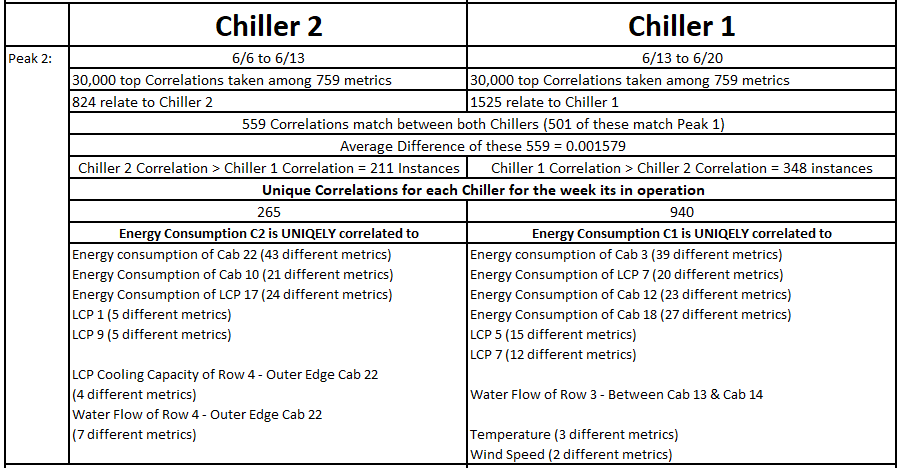
\includegraphics[scale=0.50]{peak2chillercorrelation}
\end{figure}

\begin{figure}[H]
  \caption{Correlation Analysis of each Chiller for 8/29 to 9/12}
  \label{fig:peak2chillercorrelation}
  \centering
    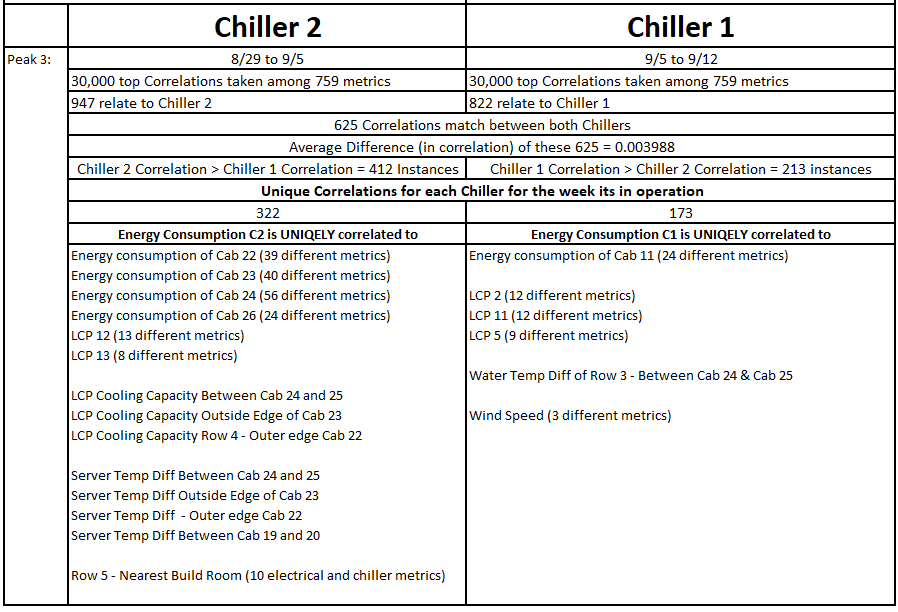
\includegraphics[scale=0.50]{peak3chillercorrelation}
\end{figure}


\section{Full list of Independent Variables for Regression Model}
\label{sec:[Full list of Independent Variables for Regression Model]}

\begin{figure}[H]
  \caption{Full list of Independent Variables used in the Regression Model}
  \label{fig:independentvariables}
  \centering
    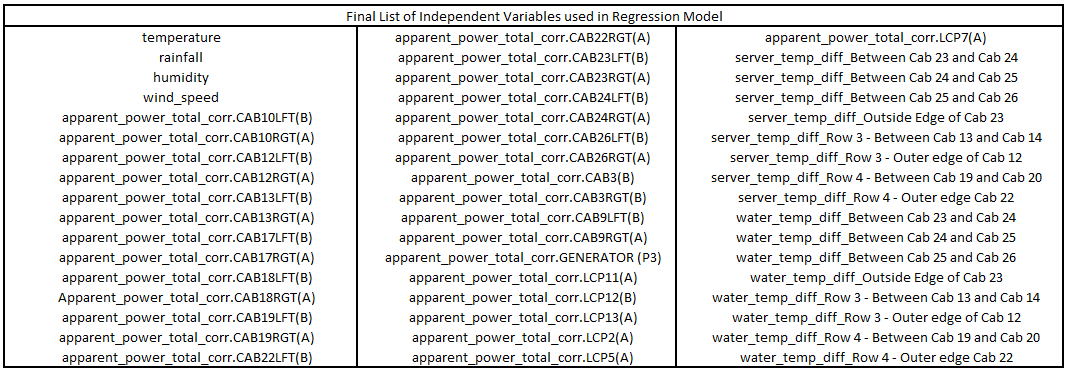
\includegraphics[scale=0.50]{independentvariables}
\end{figure} 

\section{Summary of the Output of the Regression Model}
\label{sec:[Summary of the Output of the Regression Model]}

\begin{figure}[H]
  \caption{Regression Output from Data from April 25th to May 9th}
  \label{fig:regressionresultsweek1}
  \centering
    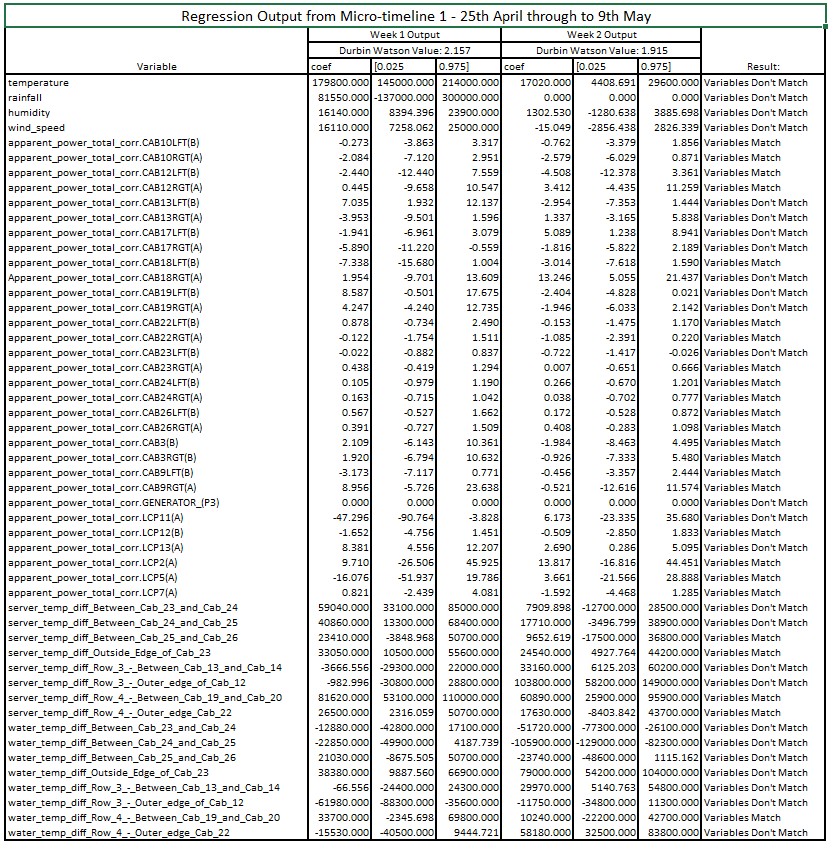
\includegraphics[scale=0.75]{regressionweek1}
\end{figure} 

\begin{figure}[H]
  \caption{Regression Output from Data from June 6th to June 20th}
  \label{fig:regressionresultsweek2}
  \centering
    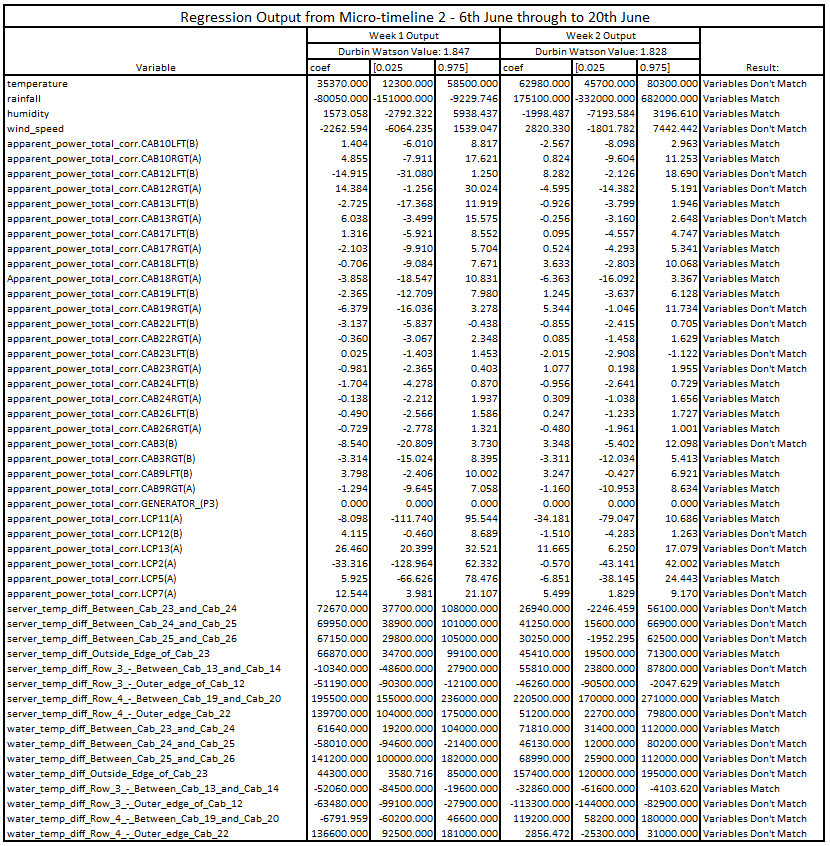
\includegraphics[scale=0.75]{regressionweek2}
\end{figure} 

\begin{figure}[H]
  \caption{Regression Output from Data from August 29th to September 12th}
  \label{fig:regressionresultsweek3}
  \centering
    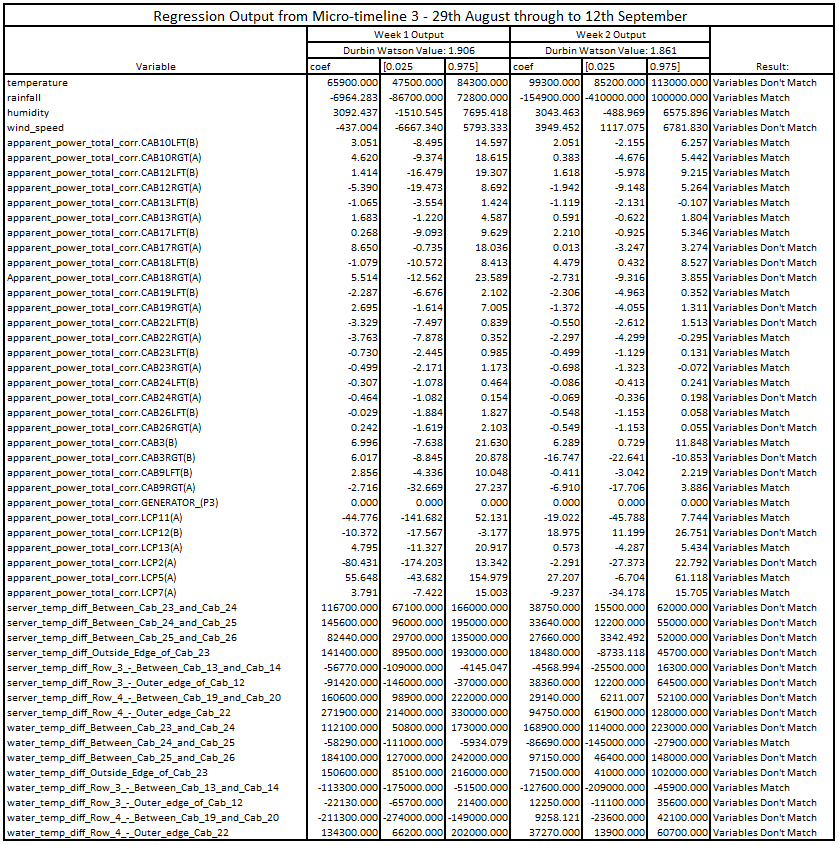
\includegraphics[scale=0.75]{regressionweek3}
\end{figure} 

\end{document}
